\begin{table*}
	\caption{Benchmark query features}\label{tab:tpch-queries}
	%\vspace{-1.2em}
	\centering
	\resizebox{\textwidth}{!}{
		\begin{tabular}{rcccccccccccccccccccccccccccccc}
			\toprule
			                 & \multicolumn{6}{c}{\qtpc}   & \multicolumn{5}{c}{\qtpce}
			                 & \multicolumn{18}{c}{\qcust}                                                                                                                                                                                                                                                                                 \\
			\cmidrule(lr){2-7} \cmidrule(lr){8-12} \cmidrule(lr){13-30}
			\textbf{Query}   & 1                           & 6                          & 7      & 9      & 12     & 19     & 1      & 3      & 4      & 12     & 15     & 1      & 2      & 3      & 4      & 5      & 6      & 7      & 8      & 9      & 10     & 11     & 12     & 13     & 14     & 15     & 16     & 17     & 18     \\
			\midrule
			\# tables joined & 1                           & 1                          & 6      & 6      & 2      & 2      & 1      & 3      & 2      & 2      & 2      & 1      & 2      & 5      & 2      & 2      & 1      & 1      & 2      & 8      & 4      & 3      & 2      & 2      & 5      & 3      & 4      & 3      & 1      \\
			\# aggregates    & 8                           & 1                          & 1      & 1      & 2      & 1      & 0      & 0      & 0      & 0      & 0      & 0      & 0      & 0      & 0      & 0      & 0      & 0      & 0      & 0      & 0      & 0      & 0      & 0      & 0      & 0      & 0      & 0      & 0      \\
			\textsf{UNION}   & \xmark                      & \xmark                     & \xmark & \xmark & \xmark & \xmark & \xmark & \xmark & \xmark & \xmark & \xmark & \xmark & \xmark & \xmark & \xmark & \xmark & \xmark & \xmark & \xmark & \xmark & \xmark & \xmark & \xmark & \xmark & \xmark & \xmark & \xmark & \xmark & \cmark \\
			\textsf{EXCEPT}  & \xmark                      & \xmark                     & \xmark & \xmark & \xmark & \xmark & \xmark & \xmark & \xmark & \xmark & \xmark & \xmark & \xmark & \xmark & \xmark & \xmark & \xmark & \xmark & \xmark & \xmark & \xmark & \xmark & \xmark & \xmark & \xmark & \xmark & \cmark & \xmark & \xmark \\
			\textsf{DISTINCT} & \xmark  					& \xmark  					& \xmark  &	\xmark  &	\xmark & \xmark  &	\xmark	&	\xmark	&	\xmark	&	\xmark	&	\xmark	& \xmark  &	\cmark  &\xmark  &	\xmark  &	\xmark  &	\xmark  & \xmark  & \xmark  & \xmark  & \xmark  & \xmark  & \xmark  &\xmark  &\xmark  & \cmark  &	\xmark  &\xmark  &\xmark \\
			\textsf{GROUP BY} & \cmark    					& \xmark 					& \cmark  &	\cmark  & \cmark  &	\xmark  &	\cmark  &\cmark  &\cmark  &\cmark  &\cmark  &	\xmark	& \xmark	&	\xmark	&	\cmark	&\xmark	&	\cmark	&\xmark	&	\xmark	&\cmark	&\cmark	&\xmark	&\xmark	&\xmark	&\cmark	&\xmark	&\xmark	&\cmark	&\xmark	\\
			\textsf{ORDER BY} & \cmark						& \xmark					& \cmark  & \cmark & \cmark & \xmark & \xmark & \xmark & \xmark & \xmark & \xmark & \xmark & \xmark & \xmark & \xmark & \xmark & \xmark & \xmark & \xmark & \xmark & \xmark & \xmark & \xmark & \xmark & \xmark & \xmark & \xmark & \xmark & \xmark \\
			\bottomrule
		\end{tabular}
	}
\end{table*}
\begin{table*}
	\caption{System comparison: supported queries on the TPC-H 1GB
		dataset (Y -- successful execution, \textcolor{red}{O} -- out of memory, \textcolor{red}{N} -- query not supported, \textcolor{red}{T} -- timeout $>3000s$)}\label{tab:sys_comp}
	%\vspace{-1.2em}
	\centering
	\resizebox{\textwidth}{!}{
		\begin{tabular}{rcccccccccccccccccccccccccccccc}
			\toprule
			                & \multicolumn{6}{c}{\qtpc}   & \multicolumn{5}{c}{\qtpce}
			                & \multicolumn{18}{c}{\qcust}                                                                                                                                                                                                                                                                                                                                                                                                \\
			\cmidrule(lr){2-7} \cmidrule(lr){8-12} \cmidrule(lr){13-30}
			\textbf{Query}  & 1                           & 6                          & 7                  & 9                  & 12                 & 19                 & 1 & 3 & 4                  & 12 & 15 & 1                  & 2 & 3 & 4                  & 5                  & 6                  & 7 & 8                  & 9                  & 10 & 11 & 12                 & 13 & 14 & 15 & 16                 & 17 & 18                 \\
			\midrule
			ProvSQL (prov.) & Y                           & Y                          & Y                  & Y                  & Y                  & Y                  & Y & Y & Y                  & Y  & Y  & Y                  & Y & Y & Y                  & Y                  & Y                  & Y & Y                  & Y                  & Y  & Y  & Y                  & Y  & Y  & Y  & Y                  & Y  & Y                  \\
			ProvSQL (prob.) & \textcolor{red}{O}          & Y                          & \textcolor{red}{O} & Y                  & Y                  & Y                  & Y & Y & Y                  & Y  & Y  & Y                  & Y & Y & Y                  & Y                  & Y                  & Y & Y                  & \textcolor{red}{O} & Y  & Y  & Y                  & Y  & Y  & Y  & Y                  & Y  & Y                  \\
			GProM           & \textcolor{red}{N}          & \textcolor{red}{N}         & \textcolor{red}{N} & \textcolor{red}{N} & \textcolor{red}{N} & \textcolor{red}{N} & Y & Y & Y                  & Y  & Y  & \textcolor{red}{O} & Y & Y & Y                  & \textcolor{red}{O} & Y                  & Y & Y                  & Y                  & Y  & Y  & \textcolor{red}{O} & Y  & Y  & Y  & \textcolor{red}{N} & Y  & \textcolor{red}{N} \\
			MayBMS          & \textcolor{red}{N}          & \textcolor{red}{N}         & \textcolor{red}{N} & \textcolor{red}{N} & \textcolor{red}{N} & \textcolor{red}{N} & Y & Y & Y                  & Y  & Y  & Y                  & Y & Y & \textcolor{red}{T} & \textcolor{red}{O} & Y                  & Y & Y                  & \textcolor{red}{O} & Y  & Y  & Y                  & Y  & Y  & Y  & \textcolor{red}{N} & Y  & \textcolor{red}{N} \\
			\bottomrule
		\end{tabular}
	}
\end{table*}


\section{Experimental Evaluation}\label{sec:experiments}

We start this section by presenting how we built our benchmark and on
which SQL queries different systems are tested. We then evaluate the performance of ProvSQL for provenance and probability computation, and compare it to GProM~\cite{bahareh2018gprom} and MayBMS~\cite{huang2009maybms}.

\subsection{Building the Benchmark}

A natural candidate for benchmarking queries in database systems is the
TPC benchmark
suite\footnote{\url{https://www.tpc.org/information/benchmarks5.asp}}. We
started with the \mbox{TPC-H} 3.0.1 database generator and its associated suite
of queries. TPC-H is a standard benchmark for decision support systems,
and includes 22 query templates that are typical of this kind of
application, including some with high computational cost.
The TPC-H schema is formed of 8 tables, 6 whose size increases proportionally
to a provided \emph{scale factor} (\texttt{lineitem}, \texttt{orders},
\texttt{part}, \texttt{supplier}, \texttt{customer}, and
\texttt{partsupp}) and 2 which are fixed (\texttt{nation} and
\texttt{region}). The scale factor allows to control the total size of
the database. A scale factor of~$k$ results in a database of roughly~$k$
GB.

None of the systems tested currently support the functionalities present
in all TPC-H queries. In particular none of them support provenance
tracking or probability computations for subqueries in
the \mintinline{sql}{WHERE} clause or
\mintinline{sql}{ORDER BY} on the result of aggregate queries. As
previously discussed, though recent versions of ProvSQL do support nested
aggregation queries, in the absence of a clear semantics of provenance
tracking for nested aggregation, we also consider such queries
out-of-scope. Only 6
queries of TPC-H work as is in at least one tested system (as it happens,
ProvSQL); this query set is denoted as \qtpc.
 This query set is
unfortunately not suitable for GProM and MayBMS as all queries include
aggregation operators, which these systems do not support.\footnote{MayBMS
	supports limited forms of summaries for probabilistic query evaluation of aggregate
	queries, with the \mintinline{sql}{ecount()} and
	\mintinline{sql}{esum()} functions but not standard SQL aggregates.
Similarly, GProm supports some form of aggregation
\cite{bahareh2018gprom}, but not in a way
compatible with semiring provenance.}

MayBMS and its query
evaluator SPROUT \cite{DBLP:conf/icde/OlteanuHK09} were also originally evaluated on
modified TPC-H queries, and MayBMS includes a benchmark of 4 such queries,
modified to remove unsupported operations\footnote{\url{https://maybms.sourceforge.net/manual/index.html}}. We
include them in a second part of our benchmark, denoted~\qtpce{}, along with TPC-H query 3, specifically modified to remove its aggregation operator (which
GProM and MayBMS do not support).

\begin{toappendix}
	\section{Generating Custom Queries using DSQGEN}
	The TPC-DS 3.2.0 dataset comes with a query generator, DSQGEN. DSQGEN
	is more flexible than the query generator from the TPC-H dataset in the sense that
	the distributions for the scalars in the queries can be written directly in the query template syntax. This allows
	us to create our own query templates for querying the TPC-H dataset easily. We then use DSQGEN to
	generate the executable query files from our query templates.

	For example let us consider a query to retrieve line items and their corresponding orders for a given ship date range on the TPC-H dataset. We will have to write the
	query template like below.
	\begin{minted}{sql}
  DEFINE SHIPDATE_MIN = RANDOM(1,121,uniform);
  DEFINE SHIPDATE_MAX = RANDOM([SHIPDATE_MIN],121,uniform);
  SELECT l.*, o.*
  FROM lineitem l, orders o
  WHERE l.l_orderkey = o.o_orderkey
  AND l.l_shipdate >= date '1994-12-01'
  - interval '[SHIPDATE_MIN]' day
  AND l.l_shipdate < date '1995-12-01'
  - interval '[SHIPDATE_MAX]' day;
  \end{minted}

	We can then use DSQGEN to generate the following executable query file from the query template for a random seed(here, 3983237069).
	\begin{minted}{sql}
  SELECT l.*, o.*
  FROM lineitem l, orders o
  WHERE l.l_orderkey = o.o_orderkey
  AND l.l_shipdate >= date '1994-12-01'
   - interval '98' day
  AND l.l_shipdate < date '1995-12-01'
   - interval '117' day;
  \end{minted}
	In this way we have written 18 different query templates following the DSQGEN query
	template syntax.
\end{toappendix}

\qtpc{} and \qtpce{} are still not representative, in that they do not cover the
full range of SQL features as implemented by provenance systems. We thus
created an additional set \qcust{} of 18 custom queries chosen to represent a wide variety of
simple query patterns, but which cover important features of the SQL language. We relied on the DSQGEN query generator from
the TPC-DS benchmark for generation because of its flexibility, but the queries are on the TPC-H
schema as well. We used \qcust{} and other subsets of our custom queries as query loads, executing them without restarting the Postgres server in between individual query runs, allowing caching.
These 18 queries include different SQL features
such as joins, varying number of aggregates, \mintinline{sql}{EXCEPT}, \mintinline{sql}{UNION}, \mintinline{sql}{DISTINCT}, \mintinline{sql}{GROUP BY}.
Table~\ref{tab:tpch-queries} shows an overview of the features of all
queries.

Table \ref{tab:sys_comp} provides a summary of which
queries are supported on every system for the lowest scale factor (1~GB):
a ``Y'' means the query runs correctly, a ``N'' is an error due to
unsupported operators, an ``O'' an out-of-memory error, and a ``T'' a
timeout at 3\,000 seconds. For ProvSQL, we distinguish between
computation of provenance and probability evaluation. We observe that
ProvSQL is able to process all three query sets; for probabilistic query
evaluation, all but three run to completion, and none of those 3 failing
queries work
in MayBMS. Other than that, a number of queries supported by ProvSQL are
either unsupported (aggregation, difference, union operators) or fail
using MayBMS or GProM. GProM in particular is particularly sensitive to
running out of memory.

\subsection{Experimental Setup}
Benchmarks were executed on a Dell Precision 7560 workstation running Debian 12
with a 11th Gen Intel(R) Core(TM) i9-11950H processor and 64GB RAM. ProvSQL and GProM used PostgreSQL 16. As MayBMS cannot be
deployed on modern systems, we had to run it under a virtual machine run
on the same machine, provided with 50 GB RAM and 8 CPU cores; the VM ran
Ubuntu 10.

We perform the benchmarks on the TPC-H 3.0.1 dataset with indexes on primary
keys (unless otherwise mentioned) for scale factors 1 to
10, i.e., with databases of size 1 to 10~GB. For experiments involving
probability computation, we modify the deterministic TPC-H database into a
tuple-independent probabilistic database by assigning a probability of
$0.5$ to every tuple of the relations involved (note that algorithms used
for exact probabilistic query evaluation in ProvSQL and MayBMS do not
depend on the actual probability values of uncertain tuples, so another
probability valuation would have given the same results in terms of
running time).

We use \mintinline{sql}{ANALYZE} to force PostgreSQL to collect
statistics about tables once each database is fully loaded.
Each experiment is run 10 times, with the database server restarted
each time, to avoid fluctuations
independent of the system's performance. Results presented are
averaged over these 10 runs.

\subsection{Benchmarking ProvSQL}

We start with evaluating the provenance tracking of ProvSQL on our benchmark queries, for three scenarios: (i) the overhead of adding provenance tracking, (ii) the scalability of different semiring instantiations, and (iii) the scalability of adding probability evaluation.

\begin{figure}[h!]
	\begin{subfigure}{\linewidth}
		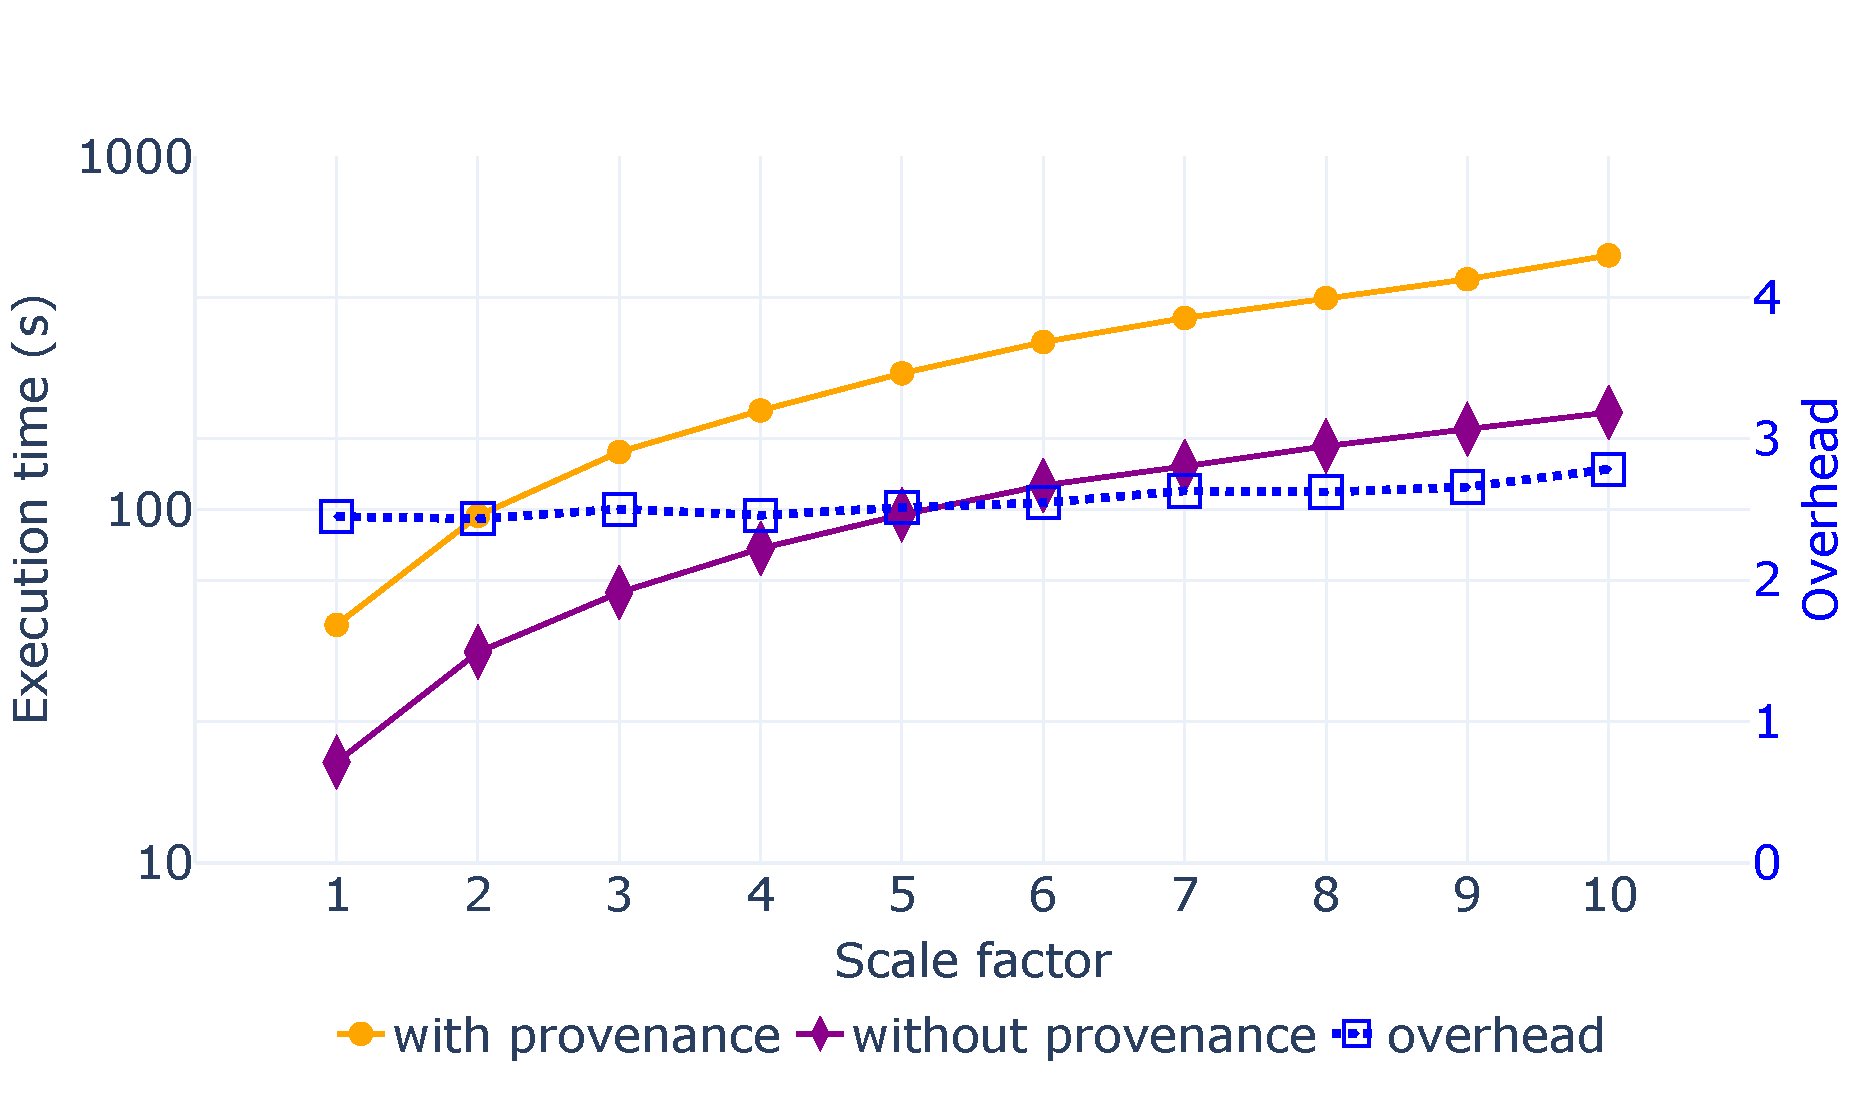
\includegraphics[width=\linewidth]{plots_pdf/overhead_qset.pdf}
		\caption{On the entire \qcust\ set}\label{fig:provsql_overhead_qset}
	\end{subfigure}
	\begin{subfigure}{\linewidth}
		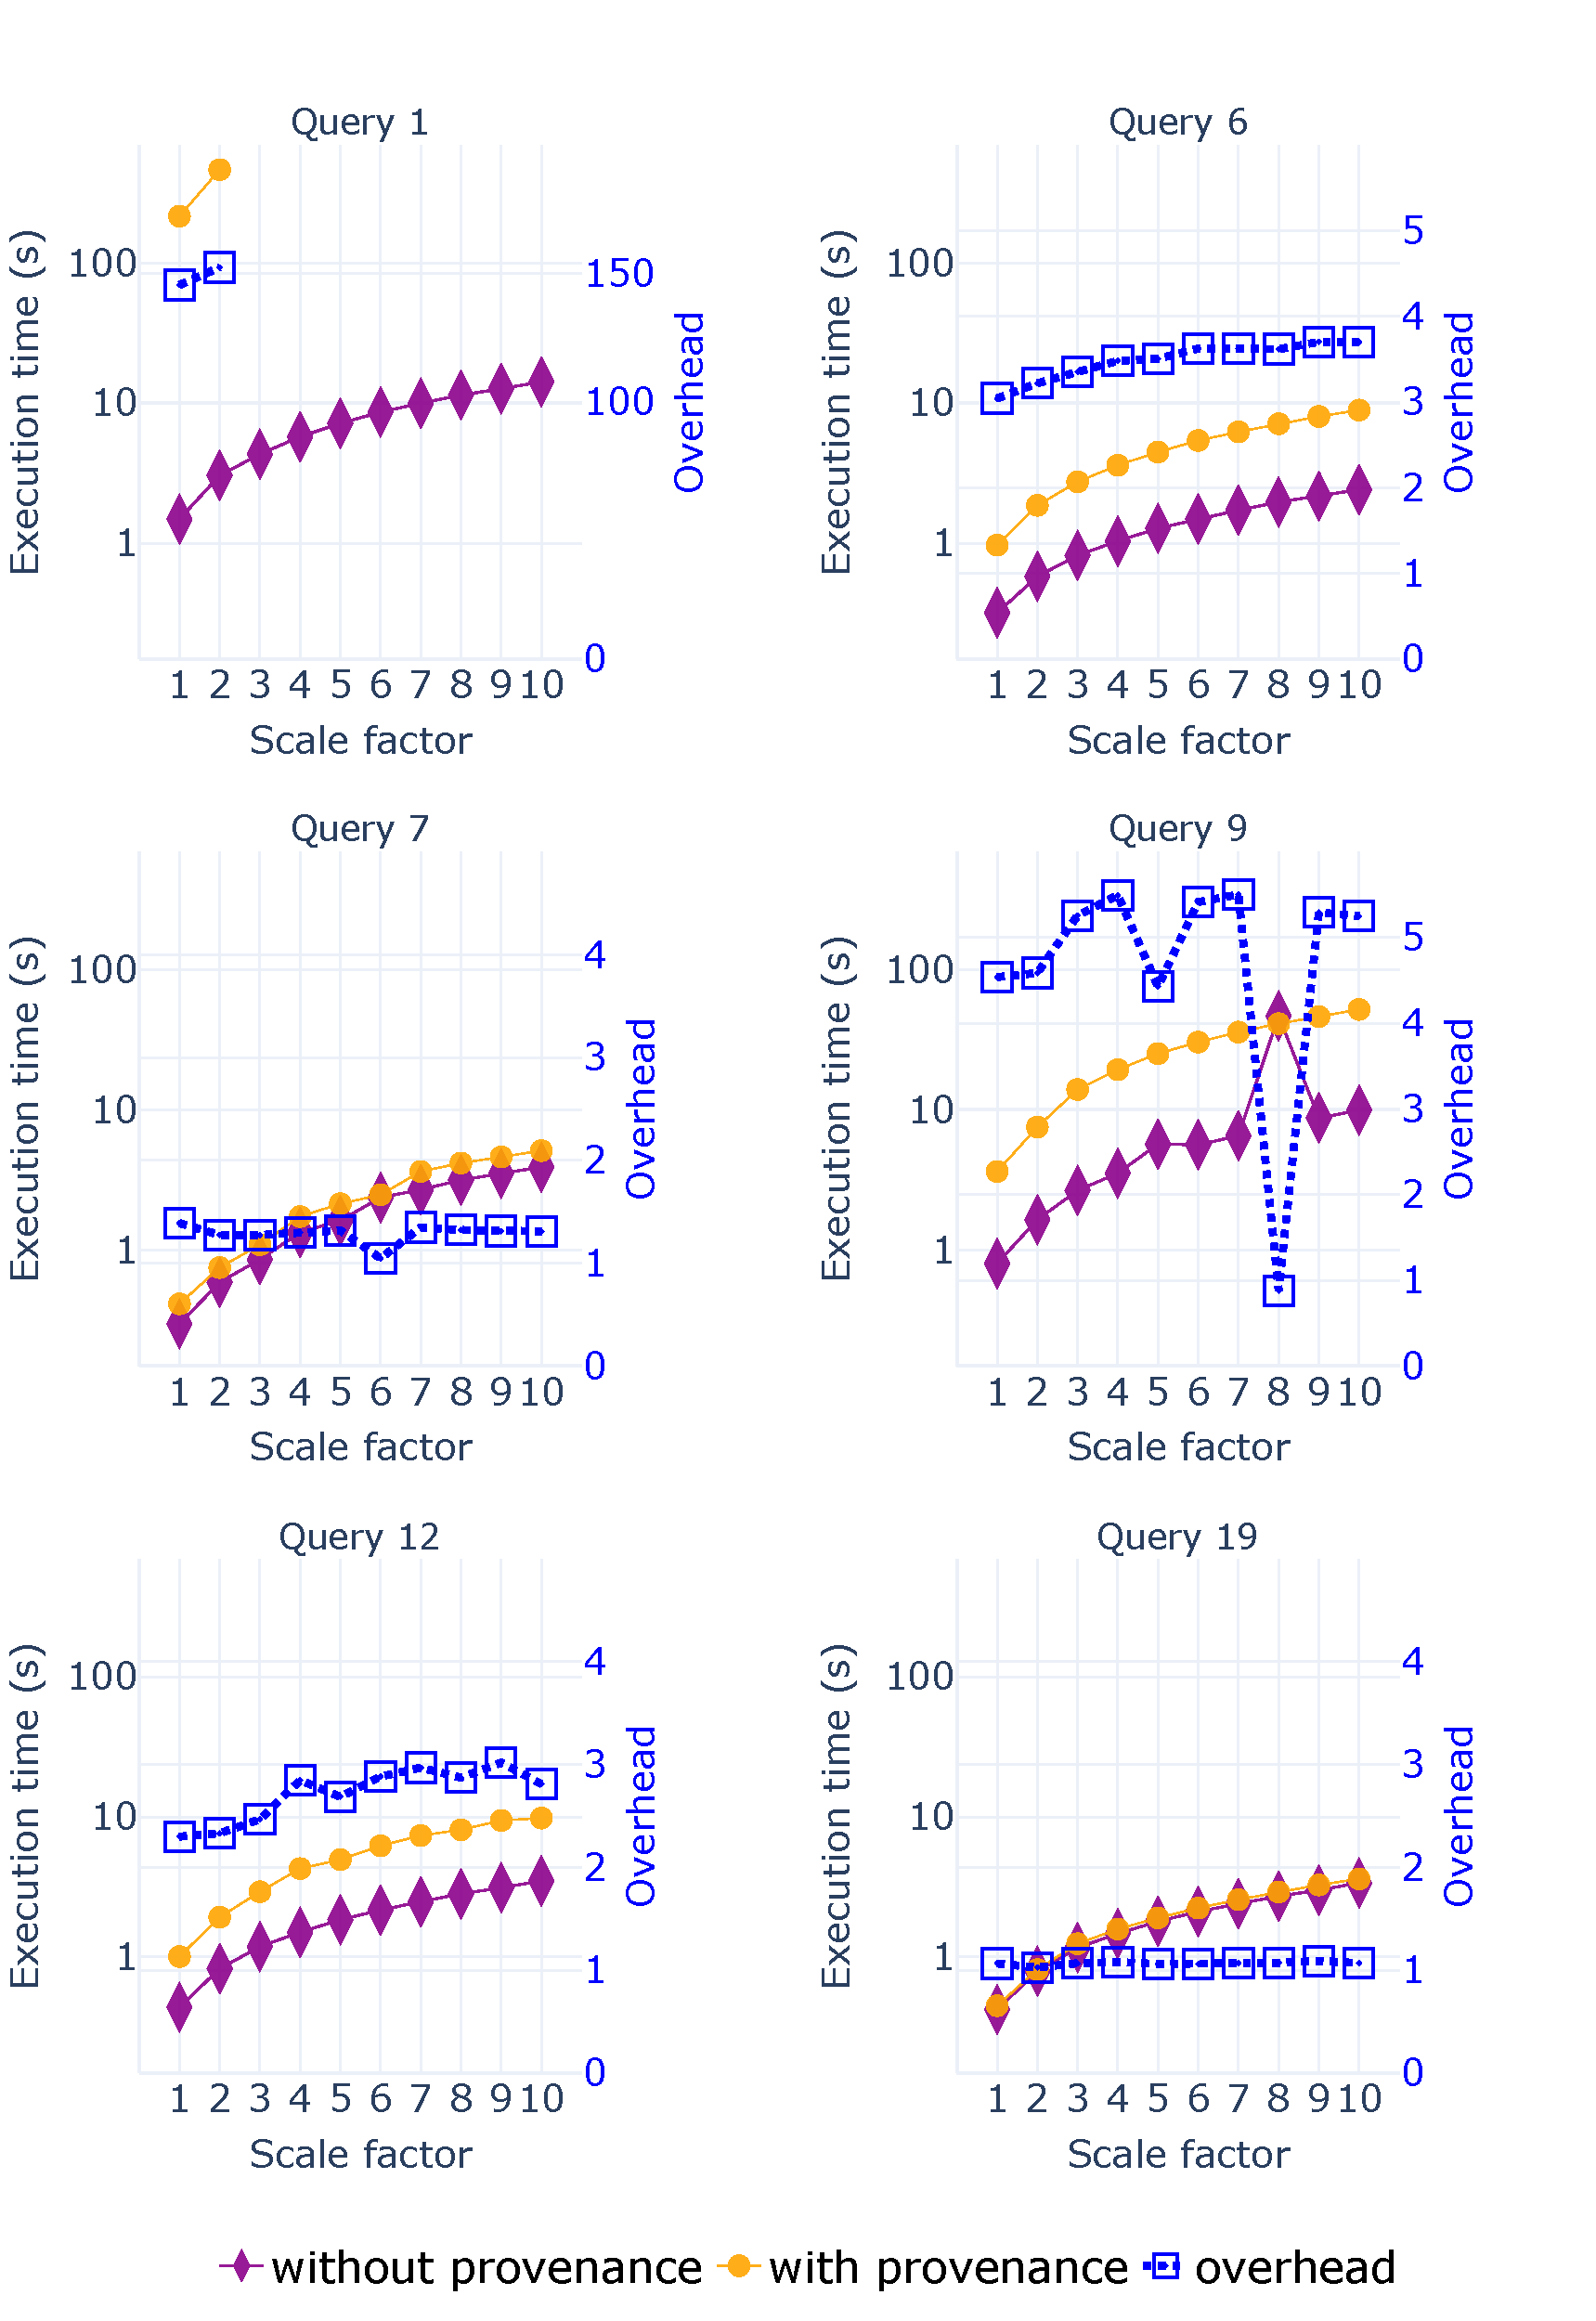
\includegraphics[width=\linewidth]{plots_pdf/overhead_tpch.pdf}
		\caption{On individual \qtpc\ queries}\label{fig:provsql_overhead_tpch}
	\end{subfigure}


	\caption{Scalability and provenance overhead: execution times (left $y$-axis, log-scale) and overhead (right $y$-axis, linear scale), at various scale factors ($x$-axis)}\label{fig:provsql_overhead}
\end{figure}



\paragraph*{Scalability and provenance overhead}
We compare the running time of queries over
PostgreSQL with the running time under ProvSQL, with provenance tracking
enabled, on TPC-H data of scale factors between 1 and 10. We are
especially interested in the overhead ratio, computed as
$\text{overhead}=\frac{t_{\text{provenance}}}{t_{\text{original}}}$.
We run the experiment on the entire \qcust query set, and on
individual queries from~\qtpc.
We show the results in Figure~\ref{fig:provsql_overhead}. Note that the blue curve corresponds
to the overhead, on the right (linear) y-axis of each plot, while the other two
curves use the left (logarithmic) y-axis.

On \qcust, Figure~\ref{fig:provsql_overhead_qset}
shows that the overhead is near-constant with the dataset size, indicating that provenance tracking scales at a similar rate as regular query execution.
This reflects the efficient implementation of provenance tracking by using provenance circuits in ProvSQL.

Results on \qtpc, Figure \ref{fig:provsql_overhead_tpch},
are of particular interest.
Query $19$ has a nearly constant overhead with little variation as the scale factor increases, characterizing efficient provenance tracking that scales independently of the database size.
For queries $7$ and $9$, we observe an anomalous \emph{decrease} in
overheads at certain scale factors due to PostgreSQL's query
optimizer adopting different execution plans when provenance tracking is
enabled, which happen to be better for that particular query. For
instance on query 9, the overhead at scale factor 8 completely
disappears. Indeed, in certain cases, provenance computation can
accidentally lead to performance improvement by guiding the PostgreSQL
optimizer to adopt a faster execution strategy. The size of the TPC-H
dataset incrementally increases with each scale factor and can cause
changes in join selectivity, indexing effectiveness and the optimizer's
cost estimates. For example, in queries $7$ and $9$ which have complex
joins, provenance tracking may force the optimizer to adopt a more
efficient join order. Except for these optimizer-driven fluctuations,
queries $7$ and $9$ have a constant overhead.
Queries $6$ and $12$ exhibit a high overhead that however remains under a
factor of~$4$, indicating scalability challenges in comparison to other
queries in this experiment. Query 6 does not involve any inner joins and
operates exclusively on the largest table in the dataset,
\texttt{lineitem}. The size of \texttt{lineitem} scales with the TPC-H
scale factor and also contains attributes with skewed, uniform, and
categorical distributions, making it a bottleneck for database optimizers
in situations where provenance tracking involves queries with a high
amount of filtering. For query $12$, the high overhead may be because of
the fact that it involves filtering conditions on aggregated tuples.
We note that ProvSQL cannot scale beyond scale factor $2$ for query~$1$ due
to memory limitations; at scale factor 1, the number of gates created in
the provenance circuit by ProvSQL for this query is
45.71M gates. For comparison, for query 7 it is 18.27k gates and
for query 9 it is 0.99M gates. Query 1 is a relatively broad query having a single filter on dates
filter along with $8$ aggregations on the
\texttt{lineitem} table, grouped on low-cardinality
columns such as \emph{l\_linestatus} and \emph{l\_returnflag}, thus limiting
scalability.
%and imposing unreasonable memory demands for higher scale factors.}


This experiment provides us with an important insight: while computing
provenance annotations generally adds overhead, this overhead is limited and even constant in most cases. It also indicates avenues for optimization of provenance computation, especially by reducing intermediate data structures.

\begin{figure}

	\begin{subfigure}{\linewidth}
		\centering
		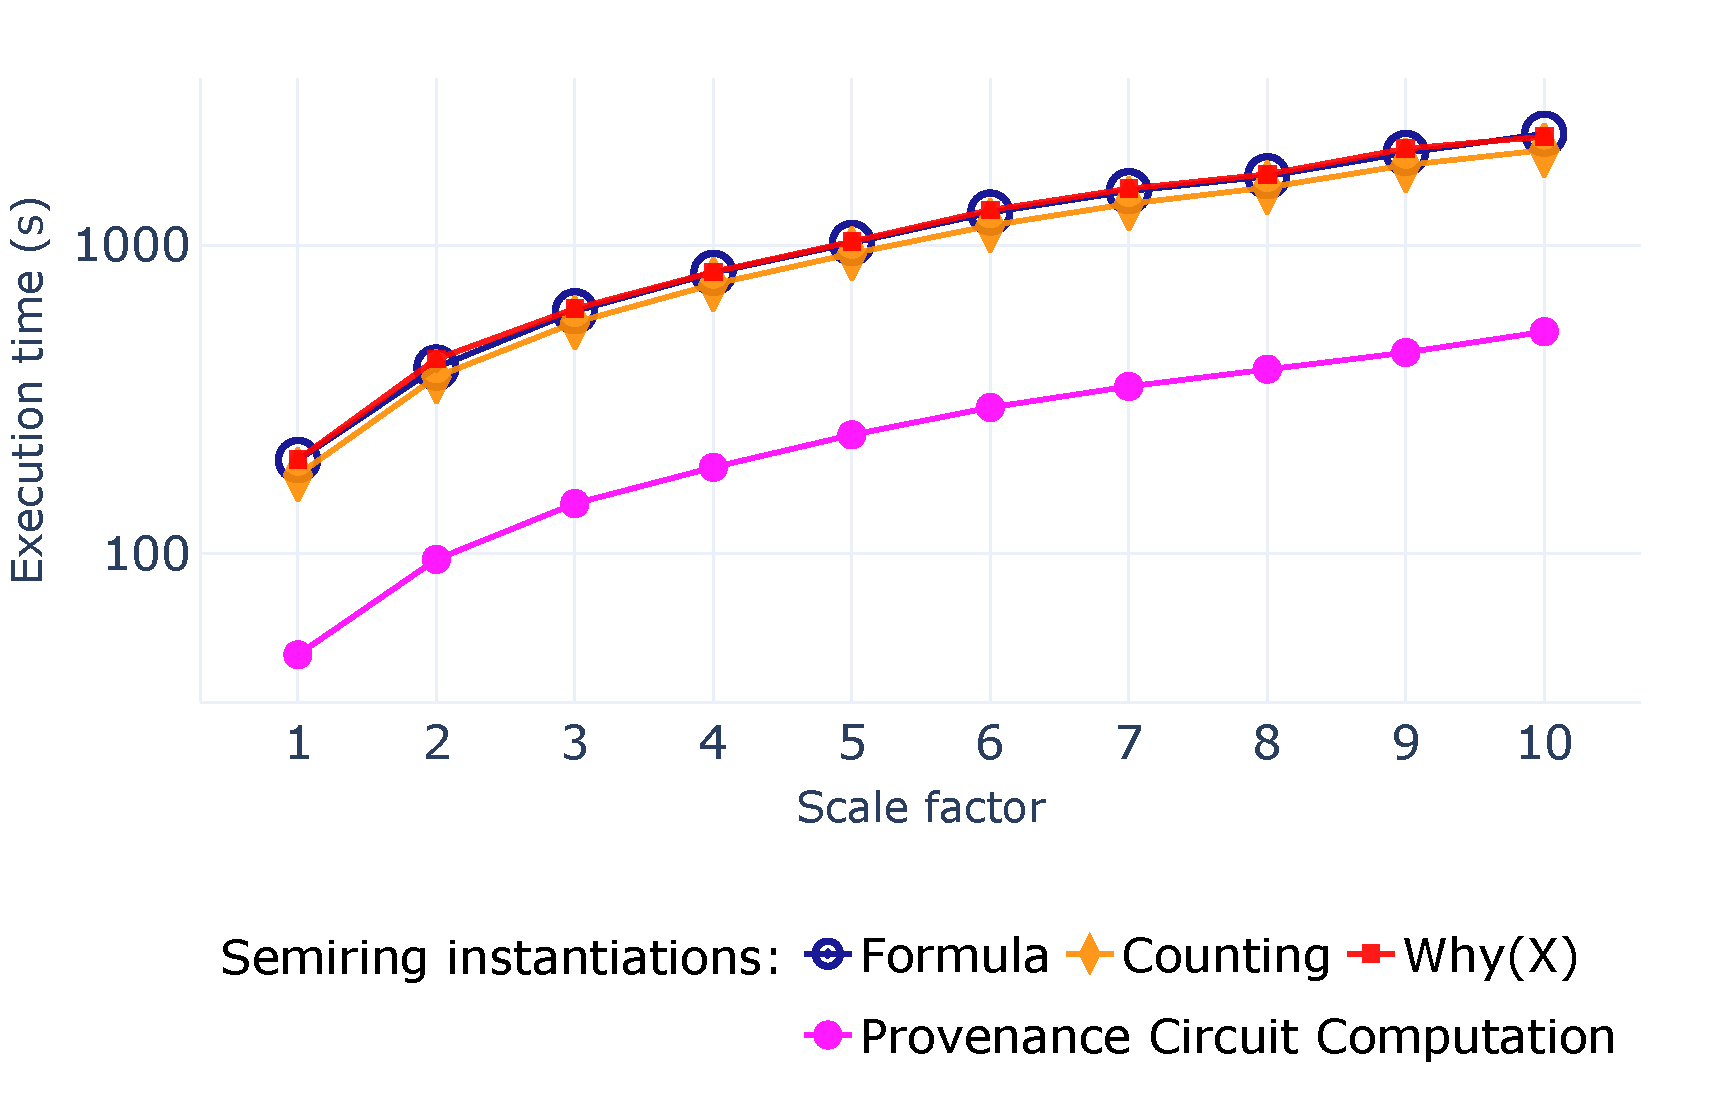
\includegraphics[width=0.8\linewidth]{plots_pdf/qset_semirings_provsql.pdf}
		\subcaption{On the entire \qcust\ set (log scale)}\label{fig:provsql_semirings_qset}
	\end{subfigure}
	\begin{subfigure}{\linewidth}
		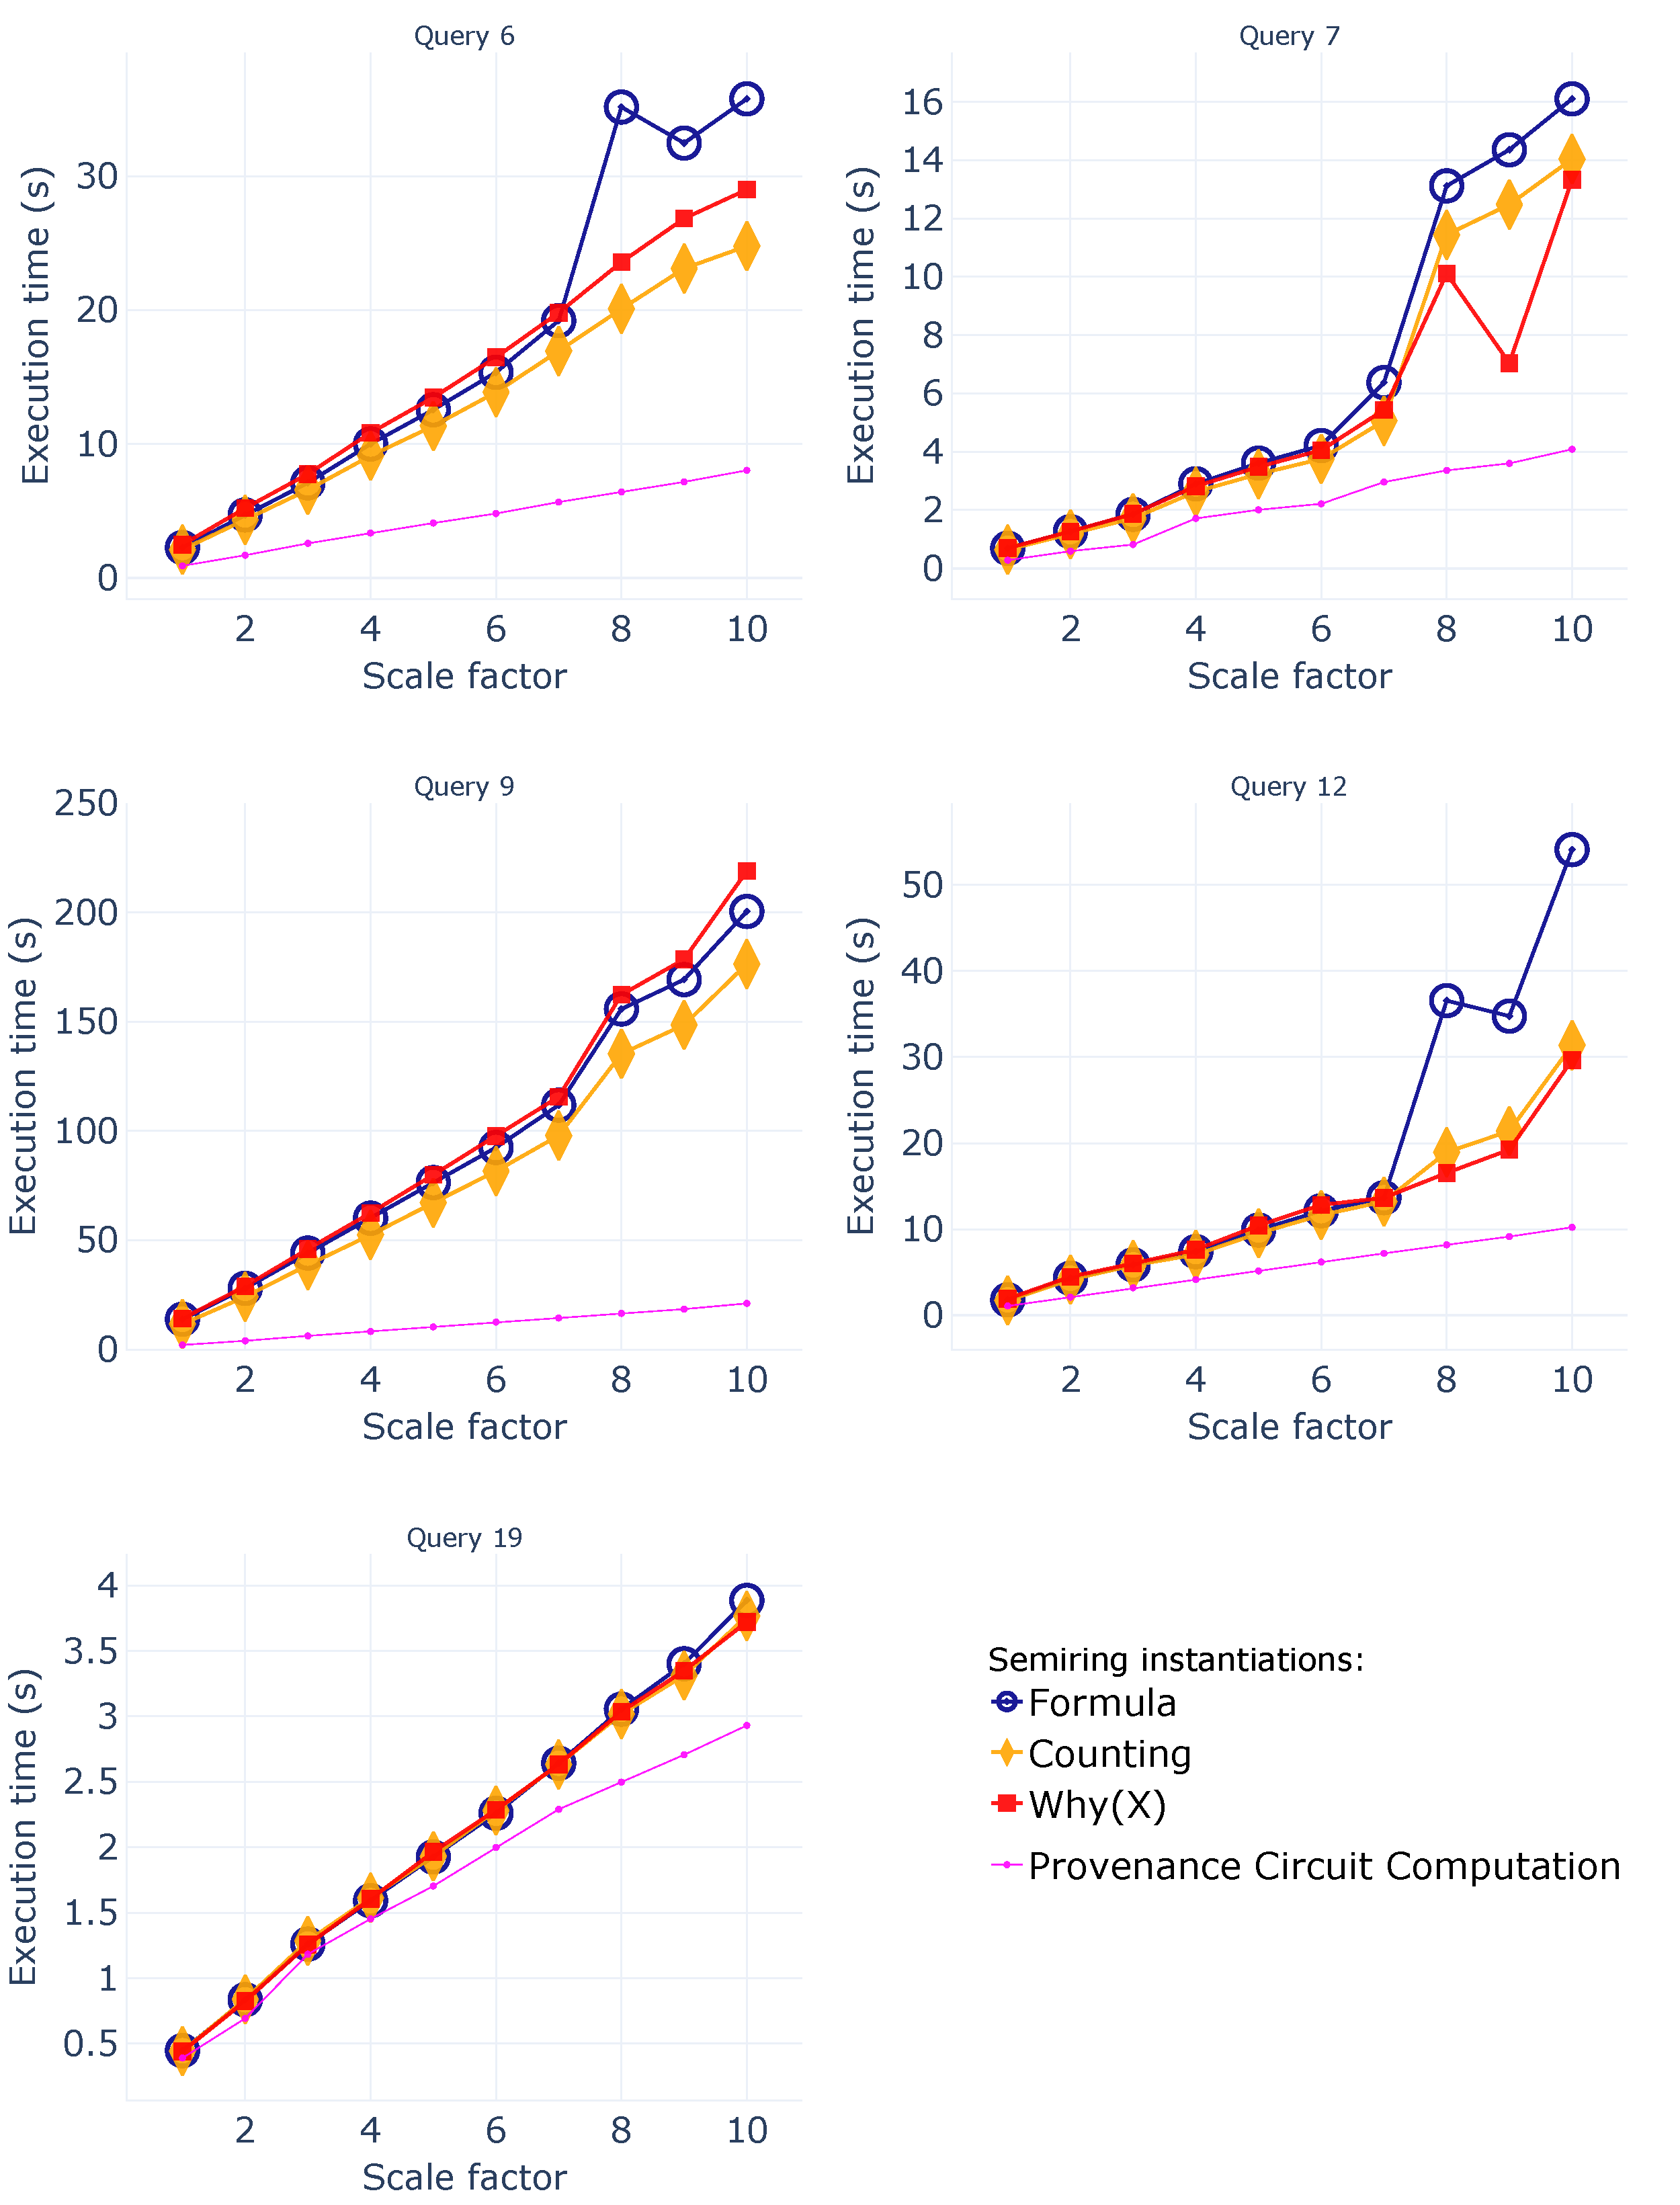
\includegraphics[width=\linewidth]{plots_pdf/semirings_tpch.pdf}
		\subcaption{On individual \qtpc\ queries  (linear scale)}\label{fig:provsql_semirings_tpch}
	\end{subfigure}


	\caption{Scalability of semiring instantiations in ProvSQL}\label{fig:provsql_semirings}
\end{figure}

\paragraph*{Semiring provenance evaluation}
We evaluate in Figure~\ref{fig:provsql_semirings} the overhead induced by
evaluating the resulting provenance circuits on different semirings
supported by ProvSQL (\emph{counting}, \emph{why-provenance}, as well as a
pseudo-semiring that just serializes in a \emph{formula}-based
representation the provenance circuit), on the TPC-H database across
scale factors 1 to 10. On the queries in \qcust\
(Figure~\ref{fig:provsql_semirings_qset}) we observe linear
trends, with the semiring instantiations across TPC-H scale factors 1 to
10. All three of the semirings introduce
virtually the same overhead to provenance computation.
The overheads observed are constant with the database size, as
none of the queries in \qcust\ have aggregates. This increased efficiency compared to aggregate provenance is due to the fact provenance computation for aggregates involves poly-sized overheads caused by
the $K-$semimodule operations.

Figure~\ref{fig:provsql_semirings_tpch} shows the overheads incurred for
individual \qtpc{} queries. We omit query 1 from \qtpc\ in this
experiment, as we just saw ProvSQL does not scale for  query 1 even when
we are only computing the provenance circuit. Except for query 9 the execution times for
the semiring instantiations indicate minimal poly-sized overheads over circuit computation times.

\paragraph*{Comparing scalability and performance queries 7 and 9 of \qtpc}
We detail the functioning of queries 7 and 9 for different implementation of ProvSQL, as we consider they are representative to some possible optimizations. Figure~\ref{fig:provsql_versions} (left) shows the scalability of three different versions of ProvSQL, implementing provenance circuits differently. Due to compatibility issues with the older implementations of circuits in ProvSQL we had to to run this experiment on PostgreSQL 14.
The current version of ProvSQL (\emph{provsql\_mmap}), which uses memory-mapped files, has the fastest running times of all three. Moreover, the running time scales linearly. The shared-memory version of ProvSQL (\emph{provsql\_shm}), in which circuits are kept in the PostgreSQL shared memory, does not scale beyond TPC-H
scale factor 4. The shared-memory implementation is also slower than the memory-mapped implementation; this is due to the impossibility to parallelize the PL/pgSQL functions that use LOCK on \emph{aggregate values}.
Although the in-database implementation of ProvSQL (\emph{provsql\_indb}), where provenance circuits are stored as PostgreSQL tables, scales linearly, it has the slowest running times.

Figure~\ref{fig:provsql_versions} (right) shows the number of gates created by ProvSQL in the provenance circuit on evaluation of the query. We can see that the number of gates created at each scale factor is significantly higher when executing query 9 of \qtpc\ than query 7. This is because, even though queries 7 and 9
 of \qtpc\ have the same number of joins and aggregations, query 9 is more selective than query 7. This also explains why the execution time for query 9 is significantly higher than query 7, and suggests that reducing the number of gates created in the provenance circuit is a good direction for future optimizations.

\begin{figure}
    \centering
        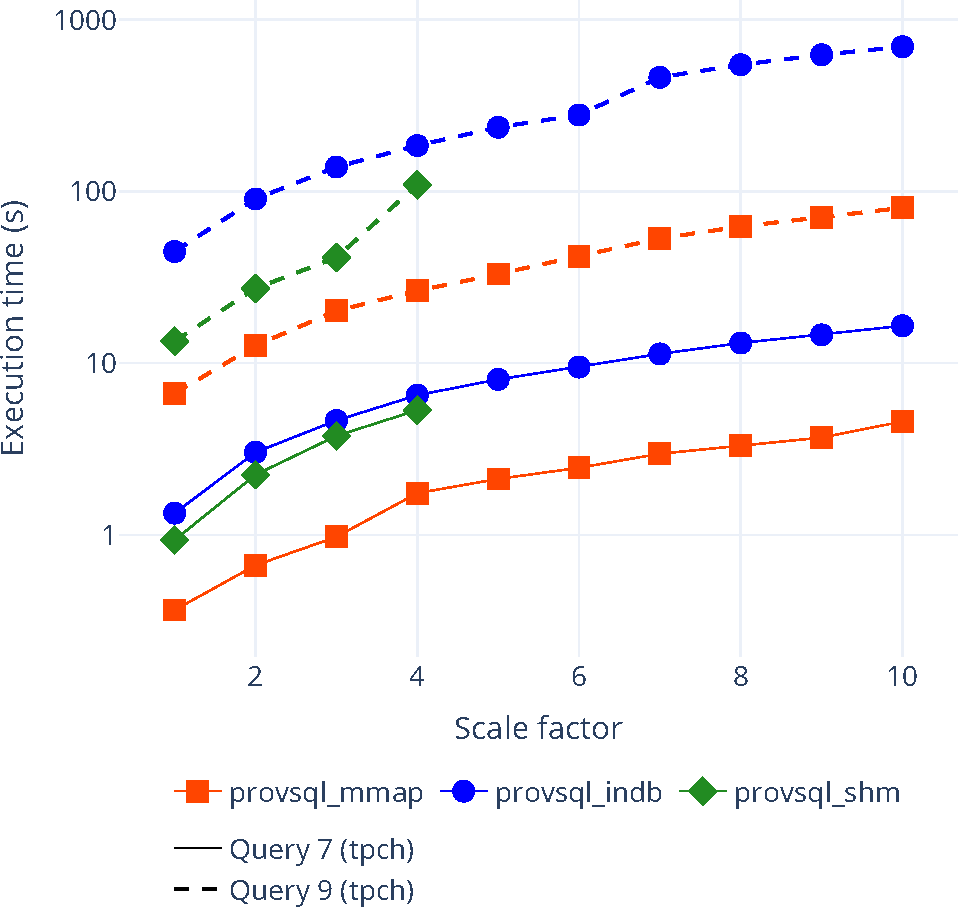
\includegraphics[width=0.48\linewidth]{plots_pdf/provsql_versions.pdf}
        \hfill
        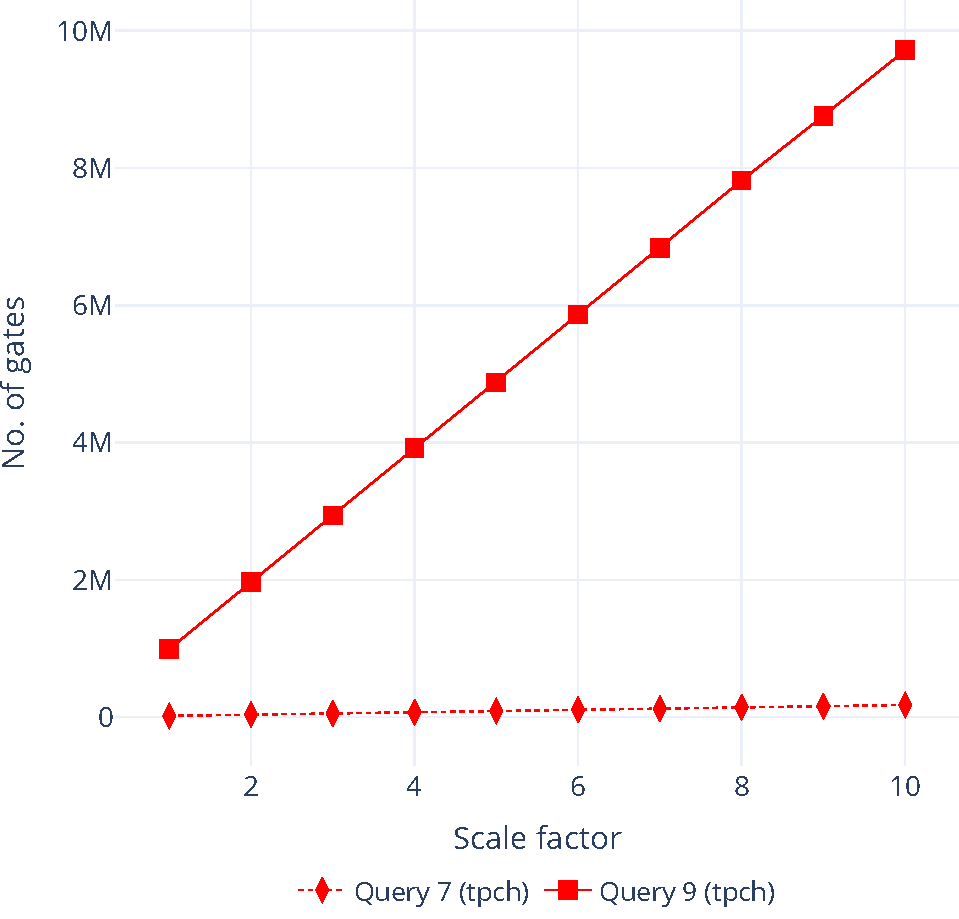
\includegraphics[width=0.48\linewidth]{plots_pdf/circuit_size_difference.pdf}
        \caption{Detailed analysis of ProvSQL on queries 7
          and 9 from \qtpc\ for different TPC-H scale factors. Left: scalability and performance of different ProvSQL
          versions (log scale). Right: number of extra gates of the provenance circuit.}
        \label{fig:provsql_versions}
\end{figure}

\begin{figure}

	\begin{subfigure}{0.4\linewidth}
		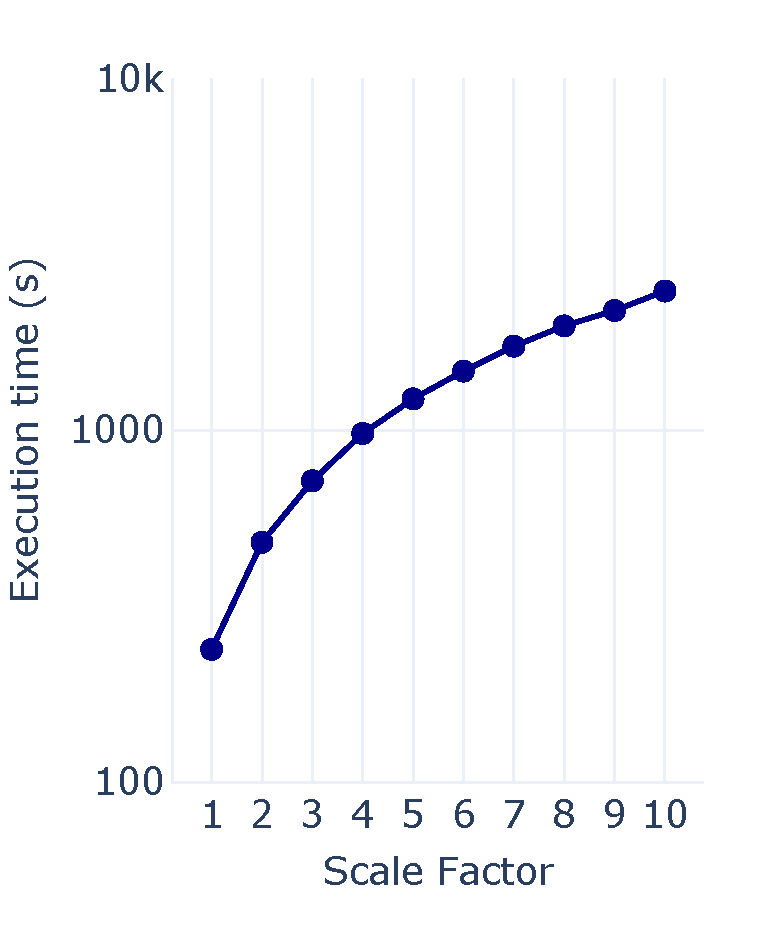
\includegraphics[width=1.2\linewidth]{plots_pdf/provsql_probab_qset.pdf}
		\subcaption{On the entire \qprob\ set (log scale)}\label{fig:provsql_prob_qset}
	\end{subfigure}%
	\hfill
	\begin{subfigure}{0.5\linewidth}
		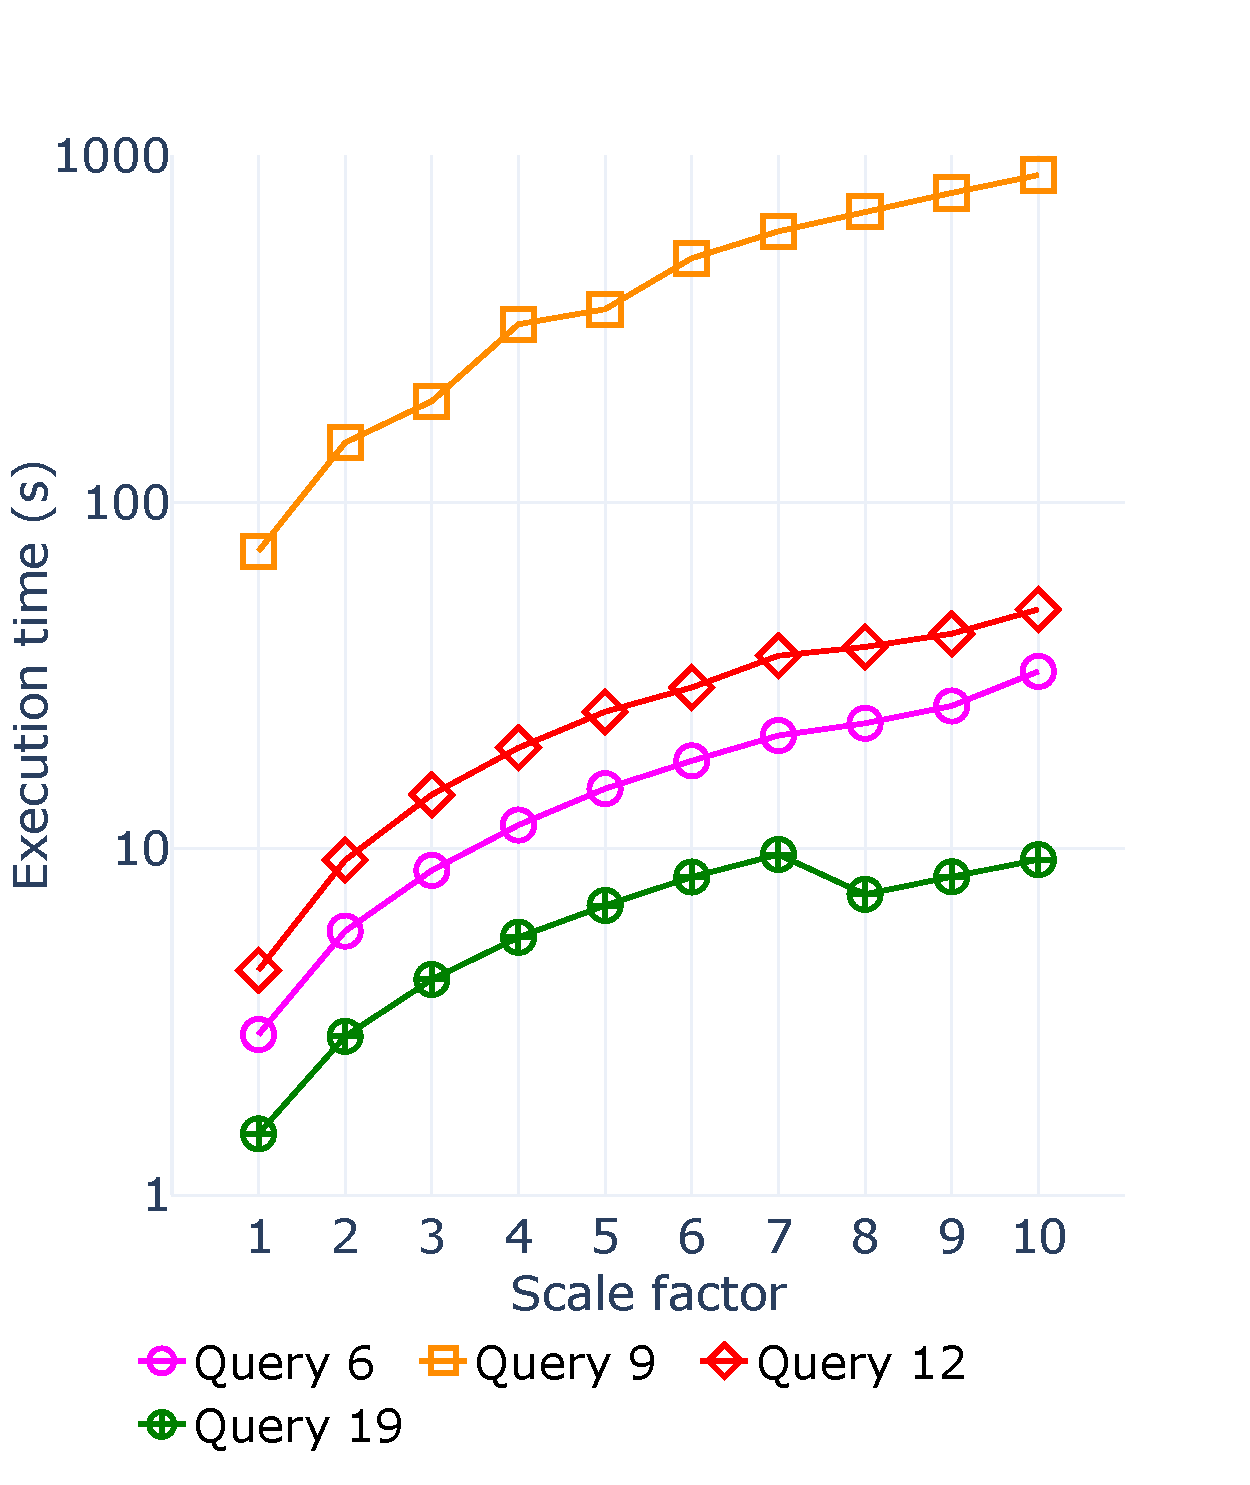
\includegraphics[width=\linewidth]{plots_pdf/probabilities_tpch_provsql.pdf}
		\subcaption{On individual \qtpc\ queries (log scale)}\label{fig:provsql_prob_tpch}
	\end{subfigure}

	\caption{Scalability of probability computation in ProvSQL}\label{fig:provsql_prob}
\end{figure}
\paragraph*{Probability evaluation}
Query 9 in \qcust\ has 8 joins and ProvSQL goes out of memory while
computing probabilities for it (more precisely, the knowledge compiler d4
called by ProvSQL runs out of memory).
We omit query 9 from \qcust\ and denote this new query set as \qprob.
Figure{~\ref{fig:provsql_prob_qset}} shows that ProvSQL scales linearly with the dataset size, when computing probabilities on query set \qprob.

Figure~\ref{fig:provsql_prob_tpch} shows generally linear scalability trends across queries 6, 9, 12, 19 from \qtpc. The exception is query 19: some optimizer driven fluctuations generate counter-intuitive performance \emph{gains} between scale factors 7 and 9. For queries 1 and 7 (not shown here) ProvSQL goes out of memory when computing probabilities, for the same reasons as outlined in the provenance overhead experiment.




\subsection{GProM vs ProvSQL for Provenance}
We now compare the performance of ProvSQL to that of GProM for computing
the provenance of query results.

\begin{figure}

		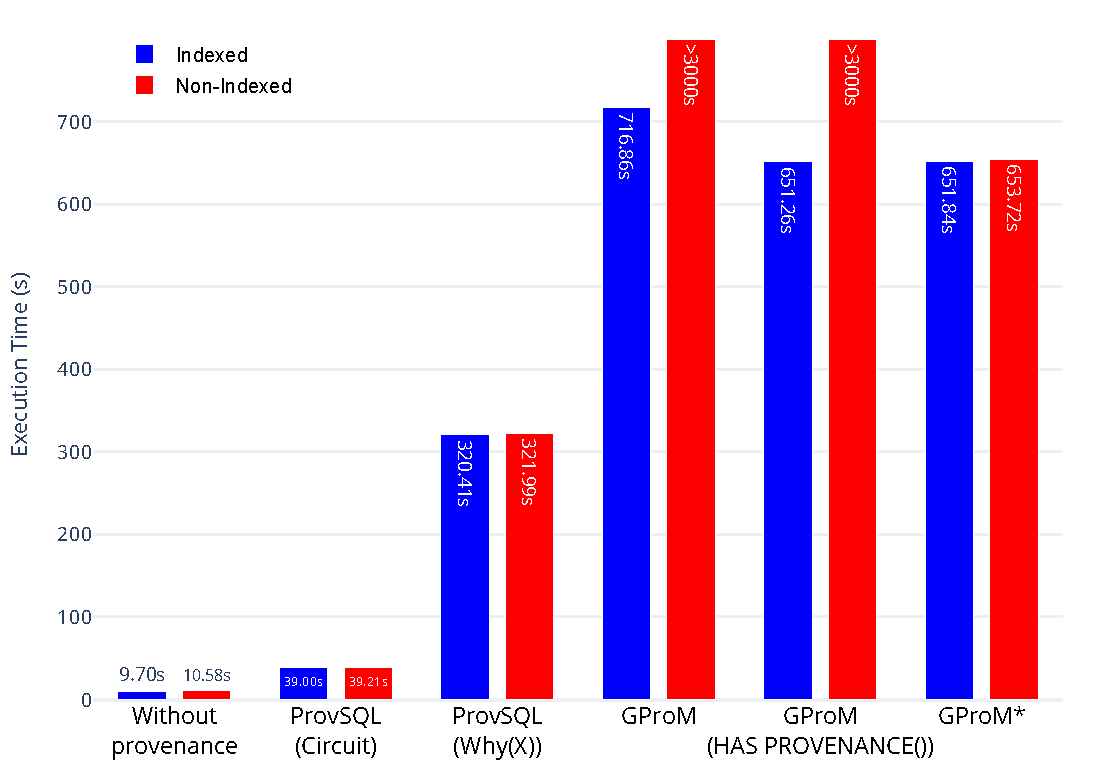
\includegraphics[width=\linewidth]{plots_pdf/indexing.pdf}
		\caption{GProM vs ProvSQL on 1 GB TPC-H dataset (with and without indexing) for \qgprom\ }\label{fig:index}

\end{figure}

We compare the execution times of provenance tracking for GProM and ProvSQL
on \qgprom, consisting of all queries in \qcust\ that GProM supports (see
Table~\ref{tab:sys_comp}) in Figure~\ref{fig:index}.
By using GProM's \mintinline{sql}{HAS PROVENANCE()} construct on the primary keys of the
tables used in a query, GProM can compute provenance expressions that closely resemble
the form of why-provenance defined in semiring-based provenance models.
However, in \mbox{TPC-H}, the primary keys are defined separately for each individual table. They cannot be used as provenance annotations because
provenance annotations, by construction, should be globally unique across the entire database.
Since GProM does not use global identifiers, we created composite primary keys for each table in the
TPC-H dataset by prefixing the table name to the primary keys and call
\mintinline{sqL}{HAS PROVENANCE()} on the composite primary keys.

We first consider the impact of indexing on the performance of these
systems.
In TPC-H, no indices (primary keys, unique constraints, etc) are defined
by default, and it is usually advised not to use indexes to compare the
performance of classical relational database systems on this dataset. In
small-scale datasets, the benefit of indexing on TPC-H queries is
actually negligible. We can observe this in Figure~\ref{fig:index} (scale
factor~1) for PostgreSQL runtime and
provenance computation using ProvSQL. However for GProM, indexing
dramatically reduces the execution time. Post-indexing, GProM yields
better results when using \mintinline{sql}{HAS PROVENANCE()}.
The bars labeled GProM$^*$ shows normalized execution
  times of GProM (with \mintinline{sql}{HAS PROVENANCE()}) rewritings, evaluated
  directly within PostgreSQL, without relying on query evaluation in
  GProM. This allows direct comparison of the query rewriting approaches
  between GproM and ProvSQL. The reported times are the total execution time of both query
  rewriting and query evaluation.


\begin{figure}
		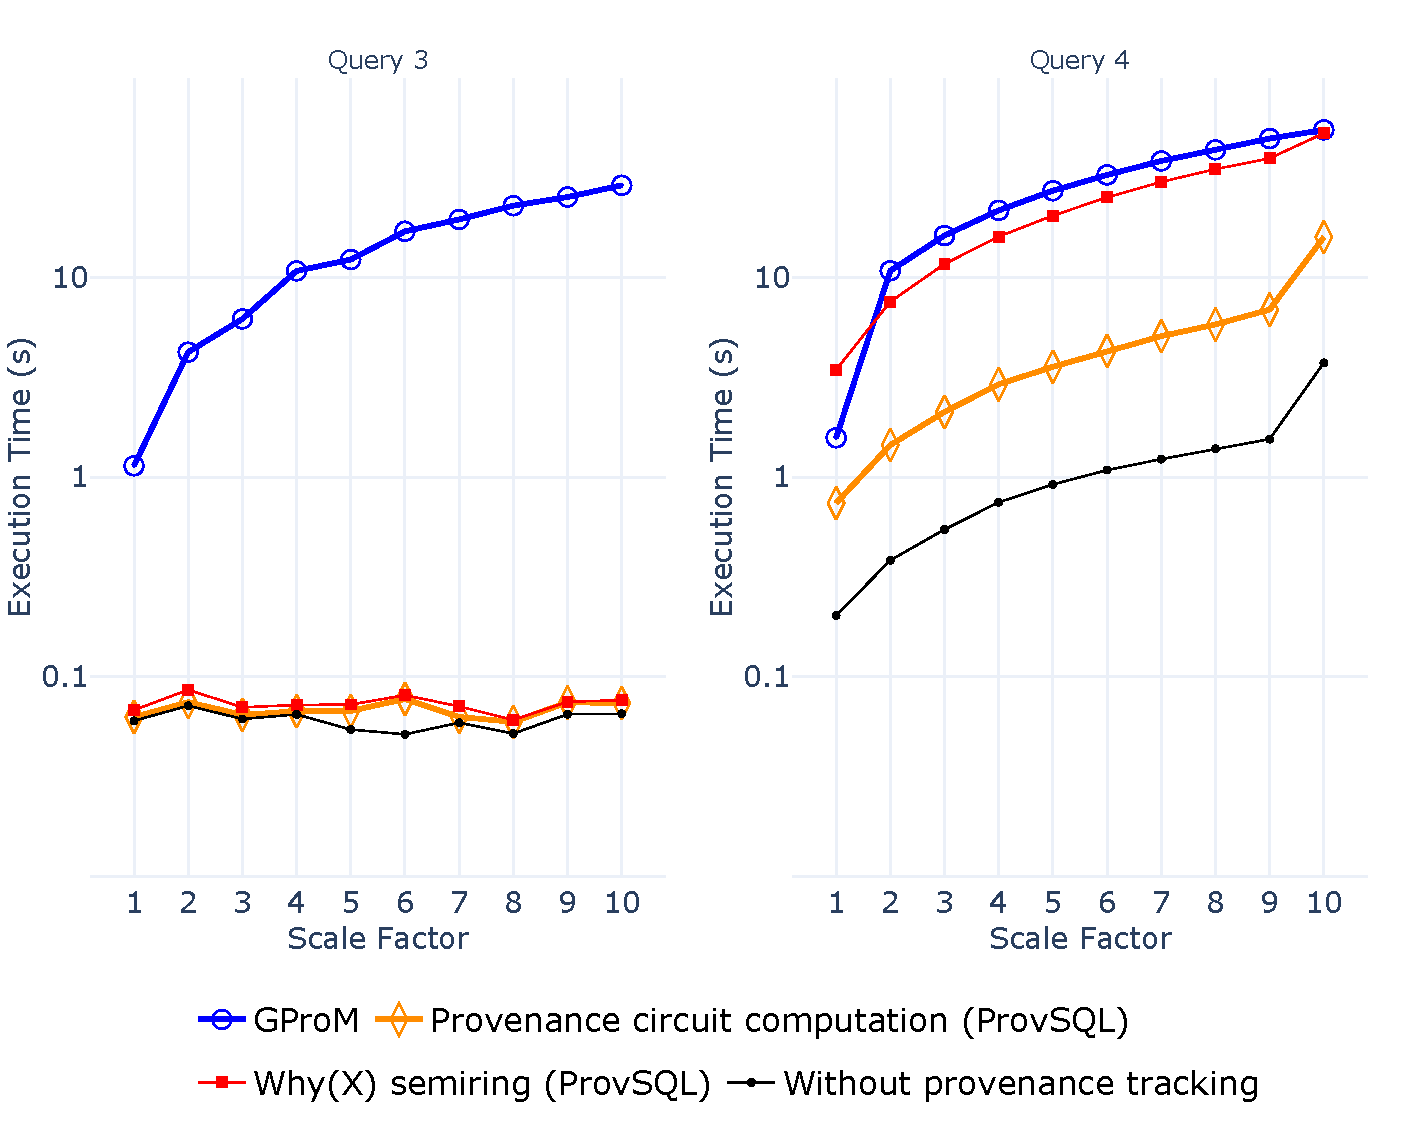
\includegraphics[width=\linewidth]{plots_pdf/gprom_tpch.pdf}
	    \caption{Scalability of GProM vs ProvSQL on query 3 and~4 from \qtpce\ (log scale)}\label{fig:gprom_tpch}
\end{figure}


In Figure~\ref{fig:gprom_tpch} we compare the scalability of provenance tracking in GProM with ProvSQL on queries 3 and 4 from \qtpce\ .
These queries are simple queries without aggregation. For query~3
the number of output tuples is limited to 20 and provenance tracking is
highly efficient across scale factors for ProvSQL. The semiring instantiations incur negligible overhead over baseline execution times
and circuit computation times. Even though GProM underperforms relatively to ProvSQL, it scales linearly.
For query 4 there are no constraints on the number of output tuples. Both ProvSQL and GProM scale linearly. The semiring instantiations in ProvSQL
incur constant overhead throughtout the scale factors. For query 4
GProM's execution times are slightly higher (except at scale factor~1).
% We compare the scalability of provenance tracking in GProM vs ProvSQL
% on \qgprom, consisting of all queries in \qcust\ that GProM supports (see
% Table~\ref{tab:sys_comp}) in Figure~\ref{fig:gprom_qset}. We outline some scalability issues with GProM.
% For scale factors 7, 8 and 9  GProM takes more than $25\,000$ seconds whereas for scale factor 10 it runs out of memory and crashes even before the timeout threshold. ProvSQL exhibits a significant overhead when it comes to provenance computation on the why-provenance semiring, but even then it scales linearly with TPC-H scale factors, unlike GProM which seems to show exponential growth in execution times.

% We zoom in on this experiment for query 3 from \qtpce\, as GProM does not
% support any of the original TPC-H queries. In Figure~\ref{fig:gprom_tpch}
% (note the y-axis is cut in two parts for readability of both
% sets of plots), we see that GProM exhibits
% exponentially increasing execution times, indicating poor scalability. At scale factor 10, GProM crashes and goes out of memory while running query 3.

% GProM's provenance representation -- discussed in detail in the supplementary material -- may be the main reason for this scalability
% issue. The size of provenance expressions (represented by extra
% attributes) can grow significantly with the number of joins. While ProvSQL benefits from efficient provenance representations, GProM's explicit tuple-level provenance annotations, by means of appending duplicates of entire tuples with renamed schema features, results in poor scalability. Although ProvSQL shows a noticeable overhead when evaluating semirings on top of the provenance circuits, it still outperforms GProM by a large margin. Moreover, Figure~\ref{fig:gprom_tpch} again shows that ProvSQL, at certain scale factors, may benefit from optimizer-driven performance improvements, as previously discussed.

\begin{figure}
	\begin{subfigure}{\linewidth}
		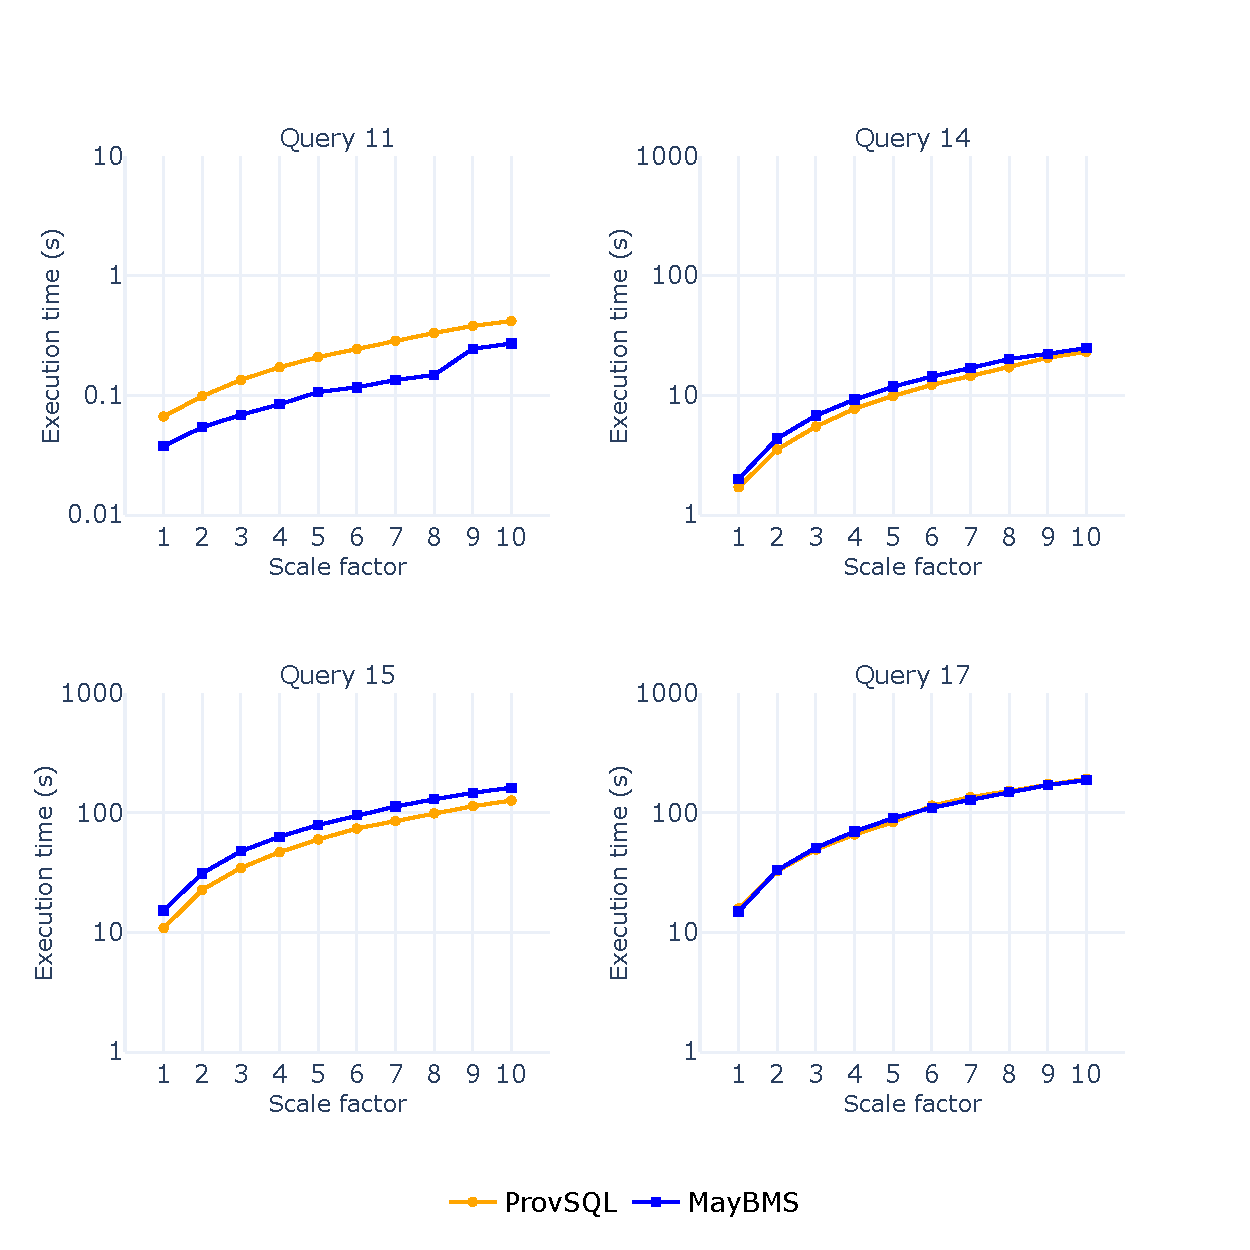
\includegraphics[width=\linewidth]{plots_pdf/unsafe.pdf}
		\subcaption{On queries 11, 14, 15 and 17 from $\mathcal{Q}^{MayBMS}$ (log scale)}\label{fig:unsafe}
	\end{subfigure}
  \vspace{-1.2em}

	\begin{subfigure}{\linewidth}
		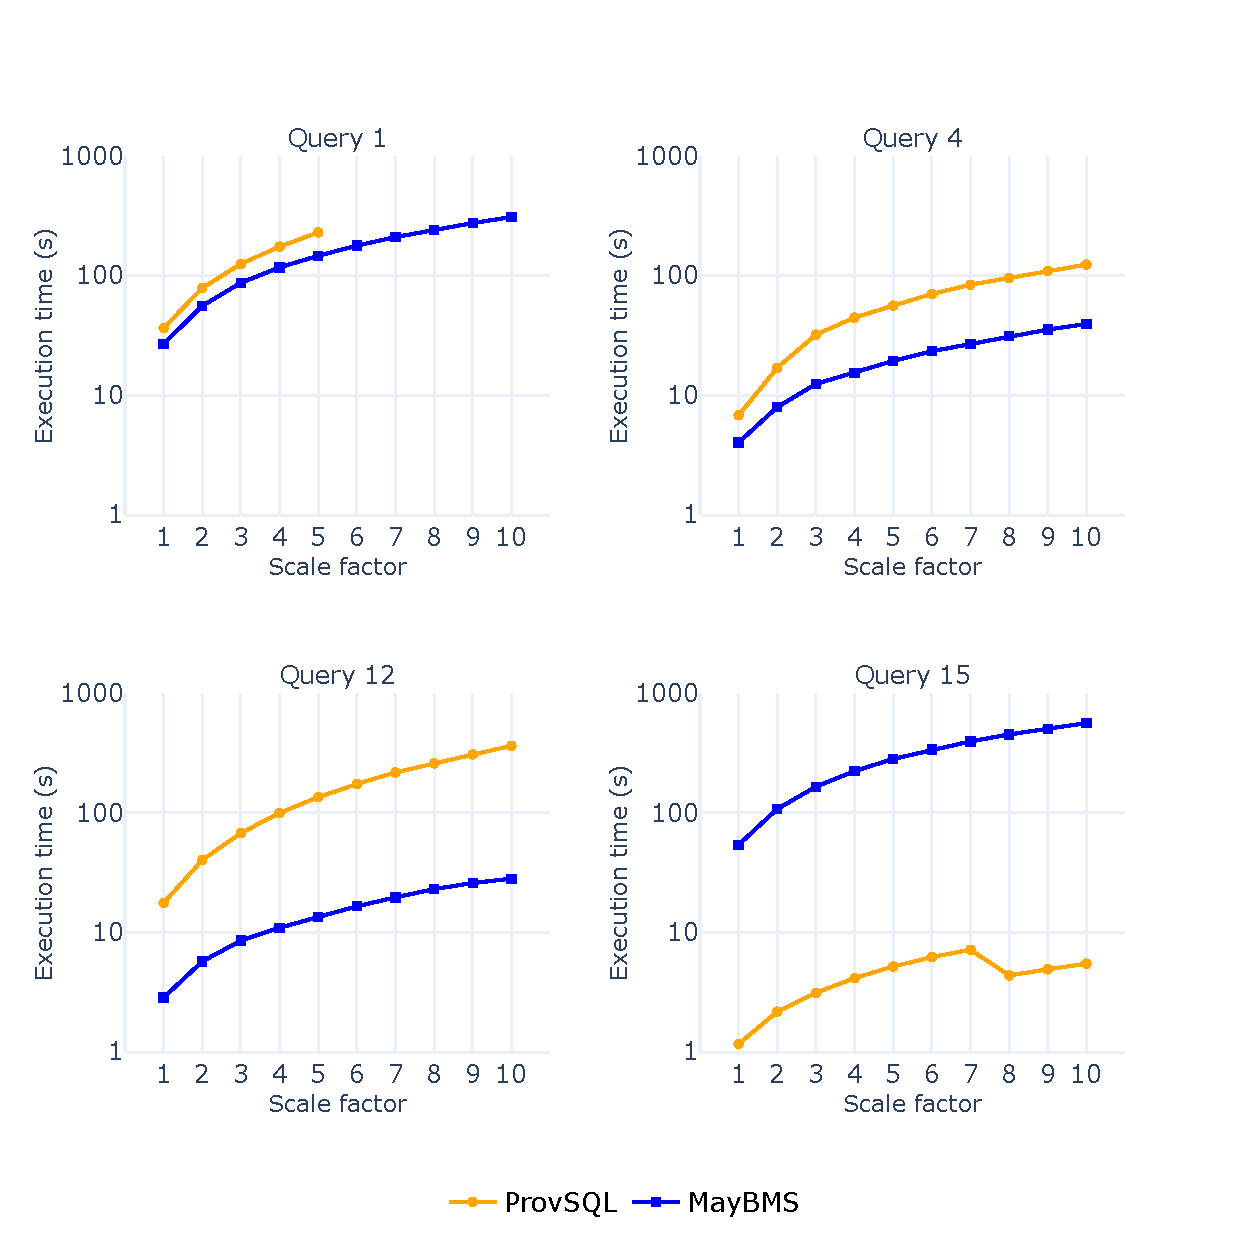
\includegraphics[width=\linewidth]{plots_pdf/maybms_provsql_tpch.pdf}
		\subcaption{On queries 1, 4, 12 and 15 from \qtpce\ (log scale)}\label{fig:safe}
	\end{subfigure}

	\caption{Scalability of MayBMS vs ProvSQL}
\end{figure}

\subsection{MayBMS vs ProvSQL for Probability}
We compare the scalability of ProvSQL and MayBMS when it comes to probability computation on uncertain tuple-independent databases, excluding queries involving set operations and aggregations, that MayBMS does not support (see Table~\ref{tab:sys_comp}).
The queries used in this experiment were rewritten
for MayBMS to adhere to the syntax constraints of this system.
%, in
%particular using
%\mintinline{sql}{conf()} and \mintinline{sql}{tconf()} were appropriate.

MayBMS implements efficient query plans for \emph{safe
	queries}~\cite{dalvi2013dichotomy}, something ProvSQL does not.
We first select 4 queries that are not safe (11, 14, 15 and 17), from our set of
custom queries for which MayBMS can compute probabilities; this query set
is denoted as \qmay.
Figure~\ref{fig:unsafe} shows that both ProvSQL and MayBMS perform similarly on all 4 queries, exhibiting linear growth with TPC-H scale factors. ProvSQL performs slightly better on queries 14 and 15; ProvSQL and MayBMS have nearly the same execution times for query 17.

We also compared ProvSQL with MayBMS by carrying out probability
computations on the modified TPC-H queries, which were used to benchmark
MayBMS. These are the largest subqueries from the original TPC-H queries
$1$, $4$, $12$, and $15$ but without aggregations and inequality joins.
Figure~\ref{fig:safe} shows how MayBMS and ProvSQL scales against the
TPC-H scale factors. For query 1, ProvSQL goes out of memory beyond scale
factor~5. Both systems scale linearly with dataset size, but MayBMS
performs noticeably better than ProvSQL on queries 1, 4 and 12. This
difference in their performance is mainly because MayBMS
and ProvSQL have different approaches when it comes to probability
evaluation. In this experiment all queries are safe and MayBMS employs
safe query plans which often results in efficient probability evaluation.
ProvSQL does not implement the safe query approach. It is designed to be
a generic system that allows provenance tracking and also offers
probability computation by means of Boolean provenance circuits. When
provenance circuits exceed manageable limits it resorts to knowledge
compilers, which may be unable to exploit the structure of the
provenance formula. In some queries, however, such as query 15, this
mechanism allows ProvSQL to compute probabilities faster than
MayBMS.

\begin{toappendix}
	\section{DSQGEN query templates for queries in \qcust}
	\begin{minted}[autogobble,fontsize=\small]{postgresql}
  -- Query 1:
  define QUANT=RANDOM(1,50,uniform);
  define MODE=TEXT({"REG AIR",1},{"AIR",1},{"RAIL",1},
  {"SHIP",1},{"TRUCK",1},{"MAIL",1},{"FOB",1});
  define DISC=RANDOM(0,10,uniform);
  SELECT l_orderkey, l_partkey, l_suppkey,
  l_linenumber, l_linestatus
  FROM lineitem
  WHERE l_shipmode = '[MODE]'
  AND l_quantity > [QUANT]
  OR l_discount >= cast([DISC] as float)/100.0;

  -- Query 2:
  define NATION=RANDOM(0,24,uniform);
  define PRICE=RANDOM(10000,100000,uniform);
  SELECT DISTINCT o.o_orderdate, o.o_custkey
  FROM orders o, customer c
  WHERE o.o_custkey = c.c_custkey
  AND o.o_totalprice > [PRICE]
  AND c.c_nationkey = [NATION]
  AND o.o_orderstatus IN ('P','F');

  -- Query 3:
  define REGION=RANDOM(0,4,uniform);
  define COST=RANDOM(1,1000,uniform);
  SELECT p.p_name, p.p_mfgr, p.p_partkey, p.p_retailprice
  FROM part p
  INNER JOIN partsupp ps ON p.p_partkey = ps.ps_partkey
  INNER JOIN supplier s  ON ps.ps_suppkey = s.s_suppkey
  INNER JOIN nation n    ON s.s_nationkey = n.n_nationkey
  INNER JOIN region r    ON n.n_regionkey = r.r_regionkey
  WHERE r.r_regionkey = [REGION]
  AND ps.ps_supplycost < [COST];

  -- Query 4:
  define PRICE=RANDOM(10000,100000,uniform);
  SELECT DISTINCT c.c_name, c.c_nationkey
  FROM customer c, orders o
  WHERE c.c_custkey = o.o_custkey
  AND o.o_totalprice > [PRICE]
  GROUP BY c.c_nationkey,c.c_name;

  -- Query 5:
  define COST=RANDOM(100,1000,uniform);
  define AVAIL=RANDOM(1,8888,uniform);
  SELECT s.s_name, s.s_address, s.s_phone
  FROM supplier s INNER JOIN partsupp ps
  ON s.s_suppkey = ps.ps_suppkey
  WHERE ps.ps_supplycost > [COST]
  OR (ps.ps_availqty > [AVAIL] AND
  ps.ps_supplycost > cast([COST] as float)/2);

  -- Query 6:
  define A=TEXT({"STANDARD",1},{"SMALL",1},{"MEDIUM",1},
  {"LARGE",1},{"ECONOMY",1},{"PROMO",1});
  define B=TEXT({"ANODIZED",1},{"BURNISHED",1},{"PLATED",1},
  {"POLISHED",1},{"BRUSHED",1});
  define C=TEXT({"TIN",1},{"NICKEL",1},{"BRASS",1},
  {"STEEL",1},{"COPPER",1});
  define SIZE=RANDOM(1,50,uniform);
  SELECT part.p_name, part.p_brand
  FROM part
  WHERE p_type = '[A] [B] [C]'
  AND p_size = [SIZE]
  GROUP BY part.p_brand, part.p_name;

  -- Query 7:
  define MODE=TEXT({"REG AIR",1},{"AIR",1},{"RAIL",1},
  {"SHIP",1},{"TRUCK",1},{"MAIL",1},{"FOB",1});
  define QUANT=RANDOM(1,50,uniform);
  SELECT *
  FROM lineitem
  WHERE l_shipmode = '[MODE]'
  AND l_quantity < [QUANT]
  AND l_linestatus = 'F';

  -- Query 8:
  define OP=TEXT({"1-URGENT",1},{"2-HIGH",1},{"3-MEDIUM",1},
  {"4-NOT SPECIFIED",1},{"5-LOW",1});
  define CLERK=RANDOM(1,9,uniform);
  SELECT c.c_name, o.o_orderdate
  FROM orders o INNER JOIN customer c ON o_custkey= c_custkey
  WHERE o_orderpriority = '[OP]'
  AND o_clerk like 'Clerk#00000000[CLERK]%';

  -- Query 9:
  define NATION=RANDOM(0,24,uniform);
  define BAL=RANDOM(1,10000,uniform);
  SELECT c.c_name, o.o_orderstatus
  FROM customer c, orders o, nation n, region r, part p,
  supplier s, partsupp ps, lineitem l
  WHERE c.c_custkey = o.o_custkey
  AND o.o_orderkey = l.l_orderkey
  AND l.l_partkey = ps.ps_partkey
  AND ps.ps_suppkey= s.s_suppkey
  AND ps.ps_partkey = p.p_partkey
  AND s.s_nationkey = n.n_nationkey
  AND n.n_regionkey = r.r_regionkey
  AND c.c_nationkey = [NATION]
  AND c_acctbal > [BAL]
  GROUP BY o.o_orderstatus, c.c_name;

  -- Query 10:
  define NATION=RANDOM(0,24,uniform);
  define BAL=RANDOM(1,10000,uniform);
  SELECT c.c_name, o.o_orderstatus
  FROM customer c, orders o, partsupp ps, lineitem l
  WHERE c.c_custkey = o.o_custkey
  AND o.o_orderkey = l.l_orderkey
  AND l.l_partkey = ps.ps_partkey
  AND c.c_nationkey = [NATION]
  AND c_acctbal > [BAL]
  GROUP BY o.o_orderstatus, c.c_name;

  -- Query 11:
  define REGION=RANDOM(0,4,uniform);
  define BAL=RANDOM(1,10000,uniform);
  SELECT s.*
  FROM supplier s
  INNER JOIN nation n ON  s.s_nationkey = n.n_nationkey
  INNER JOIN region r ON  n.n_regionkey = r.r_regionkey
  WHERE r.r_regionkey = [REGION]
  AND s.s_acctbal < [BAL];

  -- Query 12:
  define DMIN = RANDOM(1,121,uniform);
  define DMAX = RANDOM([DMIN],121,uniform);
  define TAX_A = RANDOM(0,3,uniform);
  define TAX_B = RANDOM(4,8,uniform);
  SELECT l.*, o.o_clerk, o.o_orderdate, o.o_totalprice
  FROM lineitem l INNER JOIN orders o
  ON l.l_orderkey = o.o_orderkey
  WHERE l.l_shipdate >= date '1994-12-01'
  - interval '[DMIN]' day
  AND l.l_shipdate < date '1996-12-01'
  - interval '[DMAX]' day
  AND (
  l.l_tax <= cast([TAX_A] as float)/100.0
   OR
  (l.l_tax > cast([TAX_B] as float)/100.0 AND o.o_orderstatus = 'O')
  );

  -- Query 13:
  define NATION = RANDOM(0,24,uniform);
  define P_MIN = RANDOM(10000,100000,uniform);
  define P_MAX = RANDOM([P_MIN],200000,uniform);
  SELECT c.c_name, o.o_orderstatus, c.c_nationkey, c.c_phone
  FROM customer c, orders o
  WHERE c.c_custkey = o.o_custkey
  AND c.c_nationkey = [NATION]
  AND o.o_totalprice >= [P_MIN]
  AND o.o_totalprice <= [P_MAX];

  -- Query 14:
  define REGION=RANDOM(0,4,uniform);
  define S_MIN=RANDOM(1,1000,uniform);
  define S_MAX=RANDOM([S_MIN],2000,uniform);
  SELECT s.s_name, p.p_brand, p.p_name
  FROM supplier s, partsupp ps, part p, nation n, region r
  WHERE s.s_suppkey = ps.ps_suppkey
  AND ps.ps_partkey = p.p_partkey
  AND s.s_nationkey = n.n_nationkey
  AND n.n_regionkey = r.r_regionkey
  AND r.r_regionkey = [REGION]
  AND ps.ps_supplycost >= [S_MIN]
  AND ps.ps_supplycost <= [S_MAX]
  GROUP BY p.p_brand, p.p_name, s.s_name;

  -- Query 15:
  define P_MIN = RANDOM(10000,100000,uniform);
  define P_MAX = RANDOM([P_MIN],200000,uniform);
  SELECT DISTINCT c.c_name, o.o_orderkey, l.l_linenumber
  FROM customer c, orders o, lineitem l
  WHERE c.c_custkey = o.o_custkey
  AND o.o_orderkey = l.l_orderkey
  AND o.o_totalprice >= [P_MIN]
  AND o.o_totalprice <= [P_MAX];

  --Query 16:
  define SIZE=RANDOM(1,50,uniform);
  define M=RANDOM(1,5,uniform);
  define N=RANDOM(1,5,uniform);
  SELECT c.c_name AS name, 'Customer' AS type
  FROM customer c, orders o, lineitem l, part p
  WHERE c.c_custkey = o.o_custkey
  AND o.o_orderkey = l.l_orderkey
  AND l.l_partkey = p.p_partkey
  AND p.p_size = [SIZE]
  EXCEPT
  SELECT c.c_name AS name, 'Customer' AS type
  FROM customer c, orders o, lineitem l, part p
  WHERE c.c_custkey = o.o_custkey
  AND o.o_orderkey = l.l_orderkey
  AND l.l_partkey = p.p_partkey
  AND p.p_brand = 'BRAND#[M][N]';

  -- Query 17:
  define MIN = RANDOM(1,50,uniform);
  define MAX = RANDOM([MIN],50,uniform);
  SELECT p.p_type, p.p_name, s.s_name, ps.ps_supplycost
  FROM part p, partsupp ps, supplier s
  WHERE p.p_partkey = ps.ps_partkey
  AND ps.ps_suppkey = s.s_suppkey
  AND p.p_size >= [MIN]
  AND p.p_size <= [MAX]
  GROUP BY p.p_type, p.p_name, s.s_name, ps.ps_supplycost ;

  -- Query 18:
  define NATION = RANDOM(1,25,uniform);
  SELECT c.c_name AS name, 'Customer' AS type
  FROM customer c
  WHERE c.c_nationkey = [NATION]
  UNION
  SELECT s.s_name AS name, 'Supplier' AS type
  FROM supplier s
  WHERE s.s_nationkey = [NATION];
  \end{minted}

	\section{\qtpc}
	\begin{minted}[autogobble,fontsize=\small]{postgresql}
--Query 1:
select
l_returnflag,
l_linestatus,
sum(l_quantity) as sum_qty,
sum(l_extendedprice) as sum_base_price,
sum(l_extendedprice * (1 - l_discount)) as sum_disc_price,
sum(l_extendedprice * (1 - l_discount) * (1 + l_tax)) as sum_charge,
avg(l_quantity) as avg_qty,
avg(l_extendedprice) as avg_price,
avg(l_discount) as avg_disc,
count(*) as count_order

from
	lineitem
where
	l_shipdate <= date '1998-12-01' - interval '117' day
group by
	l_returnflag,
	l_linestatus
order by
	l_returnflag,
	l_linestatus;

--Query 6:
select
	sum(l_extendedprice * l_discount) as revenue
from
	lineitem
where
	l_shipdate >= date '1995-01-01'
	and l_shipdate < date '1995-01-01' + interval '1' year
	and l_discount between 0.09 - 0.01 and 0.09 + 0.01
	and l_quantity < 24;

--Query 7:
select
	supp_nation,
	cust_nation,
	l_year,
	sum(volume) as revenue
from
	(
		select
			n1.n_name as supp_nation,
			n2.n_name as cust_nation,
			extract(year from l_shipdate) as l_year,
			l_extendedprice * (1 - l_discount) as volume
		from
			supplier,
			lineitem,
			orders,
			customer,
			nation n1,
			nation n2
		where
			s_suppkey = l_suppkey
			and o_orderkey = l_orderkey
			and c_custkey = o_custkey
			and s_nationkey = n1.n_nationkey
			and c_nationkey = n2.n_nationkey
			and (
				(n1.n_name = 'RUSSIA' and n2.n_name = 'INDIA')
				or (n1.n_name = 'INDIA' and n2.n_name = 'RUSSIA')
			)
			and l_shipdate between date '1995-01-01' and date '1996-12-31'
	) as shipping
group by
	supp_nation,
	cust_nation,
	l_year
order by
	supp_nation,
	cust_nation,
	l_year;

--Query 9:

select
	nation,
	o_year,
	sum(amount) as sum_profit
from
	(
		select
			n_name as nation,
			extract(year from o_orderdate) as o_year,
			l_extendedprice * (1 - l_discount) - ps_supplycost * l_quantity as amount
		from
			part,
			supplier,
			lineitem,
			partsupp,
			orders,
			nation
		where
			s_suppkey = l_suppkey
			and ps_suppkey = l_suppkey
			and ps_partkey = l_partkey
			and p_partkey = l_partkey
			and o_orderkey = l_orderkey
			and s_nationkey = n_nationkey
			and p_name like '%orchid%'
	) as profit
group by
	nation,
	o_year
order by
	nation,
	o_year desc;


--Query 12:
select
	l_shipmode,
	sum(case
		when o_orderpriority = '1-URGENT'
			or o_orderpriority = '2-HIGH'
			then 1
		else 0
	end) as high_line_count,
	sum(case
		when o_orderpriority <> '1-URGENT'
			and o_orderpriority <> '2-HIGH'
			then 1
		else 0
	end) as low_line_count
from
	orders,
	lineitem
where
	o_orderkey = l_orderkey
	and l_shipmode in ('TRUCK', 'AIR')
	and l_commitdate < l_receiptdate
	and l_shipdate < l_commitdate
	and l_receiptdate >= date '1997-01-01'
	and l_receiptdate < date '1997-01-01' + interval '1' year
group by
	l_shipmode
order by
	l_shipmode;

--Query 19:
select
	sum(l_extendedprice* (1 - l_discount)) as revenue
from
	lineitem,
	part
where
	(
		p_partkey = l_partkey
		and p_brand = 'Brand#54'
		and p_container in ('SM CASE', 'SM BOX', 'SM PACK', 'SM PKG')
		and l_quantity >= 4 and l_quantity <= 4 + 10
		and p_size between 1 and 5
		and l_shipmode in ('AIR', 'AIR REG')
		and l_shipinstruct = 'DELIVER IN PERSON'
	)
	or
	(
		p_partkey = l_partkey
		and p_brand = 'Brand#51'
		and p_container in ('MED BAG', 'MED BOX', 'MED PKG', 'MED PACK')
		and l_quantity >= 11 and l_quantity <= 11 + 10
		and p_size between 1 and 10
		and l_shipmode in ('AIR', 'AIR REG')
		and l_shipinstruct = 'DELIVER IN PERSON'
	)
	or
	(
		p_partkey = l_partkey
		and p_brand = 'Brand#21'
		and p_container in ('LG CASE', 'LG BOX', 'LG PACK', 'LG PKG')
		and l_quantity >= 28 and l_quantity <= 28 + 10
		and p_size between 1 and 15
		and l_shipmode in ('AIR', 'AIR REG')
		and l_shipinstruct = 'DELIVER IN PERSON'
	);
  \end{minted}

	\section{\qtpce}

		\begin{minted}[autogobble,fontsize=\small]{postgresql}
--Query1
SELECT l_returnflag, l_linestatus FROM
lineitem WHERE l_shipdate<=date '1998-09-01' GROUP BY l_returnflag, l_linestatus;

--Query3
 SELECT l_orderkey FROM customer, orders, lineitem
 WHERE c_mktsegment='BUILDING' AND c_custkey=o_custkey AND
 l_orderkey=o_orderkey AND o_orderdate<date '1995-03-15' AND
 l_shipdate>date '1995-05-15' GROUP BY l_orderkey,
 o_orderdate, o_shippriority LIMIT 20;

--Query 4
 SELECT o_orderpriority FROM orders, lineitem
 WHERE o_orderdate>=date '1993-07-01' AND o_orderdate<date '1993-10-01'
 AND l_orderkey=o_orderkey AND
 l_commitdate<l_receiptdate GROUP BY o_orderpriority;


--Query12
 SELECT l_shipmode FROM orders, lineitem WHERE
 o_orderkey=l_orderkey AND ( l_shipmode='MAIL' OR l_shipmode='SHIP' )
 AND l_commitdate<l_receiptdate AND
 l_shipdate<l_commitdate AND l_receiptdate>='1992-01-01'
 AND l_receiptdate<'1999-01-01'
 GROUP BY l_shipmode;


--Query 15
 SELECT s_suppkey, s_name, s_address, s_phone
 FROM supplier, lineitem WHERE s_suppkey=l_suppkey
 AND l_shipdate>=date '1991-10-10' AND
 l_shipdate<date '1992-01-10' GROUP BY s_suppkey, s_name, s_address, s_phone;
                    \end{minted}


\end{toappendix}
